\documentclass[]{article}
\usepackage{lmodern}
\usepackage{amssymb,amsmath}
\usepackage{ifxetex,ifluatex}
\usepackage{fixltx2e} % provides \textsubscript
\ifnum 0\ifxetex 1\fi\ifluatex 1\fi=0 % if pdftex
  \usepackage[T1]{fontenc}
  \usepackage[utf8]{inputenc}
\else % if luatex or xelatex
  \ifxetex
    \usepackage{mathspec}
  \else
    \usepackage{fontspec}
  \fi
  \defaultfontfeatures{Ligatures=TeX,Scale=MatchLowercase}
\fi
% use upquote if available, for straight quotes in verbatim environments
\IfFileExists{upquote.sty}{\usepackage{upquote}}{}
% use microtype if available
\IfFileExists{microtype.sty}{%
\usepackage{microtype}
\UseMicrotypeSet[protrusion]{basicmath} % disable protrusion for tt fonts
}{}
\usepackage[margin=1in]{geometry}
\usepackage{hyperref}
\hypersetup{unicode=true,
            pdftitle={ML Pipeline Project Code},
            pdfauthor={Lauren Rost, Mridul Singh Gangawar, Nikita Setia},
            pdfborder={0 0 0},
            breaklinks=true}
\urlstyle{same}  % don't use monospace font for urls
\usepackage{color}
\usepackage{fancyvrb}
\newcommand{\VerbBar}{|}
\newcommand{\VERB}{\Verb[commandchars=\\\{\}]}
\DefineVerbatimEnvironment{Highlighting}{Verbatim}{commandchars=\\\{\}}
% Add ',fontsize=\small' for more characters per line
\usepackage{framed}
\definecolor{shadecolor}{RGB}{248,248,248}
\newenvironment{Shaded}{\begin{snugshade}}{\end{snugshade}}
\newcommand{\KeywordTok}[1]{\textcolor[rgb]{0.13,0.29,0.53}{\textbf{#1}}}
\newcommand{\DataTypeTok}[1]{\textcolor[rgb]{0.13,0.29,0.53}{#1}}
\newcommand{\DecValTok}[1]{\textcolor[rgb]{0.00,0.00,0.81}{#1}}
\newcommand{\BaseNTok}[1]{\textcolor[rgb]{0.00,0.00,0.81}{#1}}
\newcommand{\FloatTok}[1]{\textcolor[rgb]{0.00,0.00,0.81}{#1}}
\newcommand{\ConstantTok}[1]{\textcolor[rgb]{0.00,0.00,0.00}{#1}}
\newcommand{\CharTok}[1]{\textcolor[rgb]{0.31,0.60,0.02}{#1}}
\newcommand{\SpecialCharTok}[1]{\textcolor[rgb]{0.00,0.00,0.00}{#1}}
\newcommand{\StringTok}[1]{\textcolor[rgb]{0.31,0.60,0.02}{#1}}
\newcommand{\VerbatimStringTok}[1]{\textcolor[rgb]{0.31,0.60,0.02}{#1}}
\newcommand{\SpecialStringTok}[1]{\textcolor[rgb]{0.31,0.60,0.02}{#1}}
\newcommand{\ImportTok}[1]{#1}
\newcommand{\CommentTok}[1]{\textcolor[rgb]{0.56,0.35,0.01}{\textit{#1}}}
\newcommand{\DocumentationTok}[1]{\textcolor[rgb]{0.56,0.35,0.01}{\textbf{\textit{#1}}}}
\newcommand{\AnnotationTok}[1]{\textcolor[rgb]{0.56,0.35,0.01}{\textbf{\textit{#1}}}}
\newcommand{\CommentVarTok}[1]{\textcolor[rgb]{0.56,0.35,0.01}{\textbf{\textit{#1}}}}
\newcommand{\OtherTok}[1]{\textcolor[rgb]{0.56,0.35,0.01}{#1}}
\newcommand{\FunctionTok}[1]{\textcolor[rgb]{0.00,0.00,0.00}{#1}}
\newcommand{\VariableTok}[1]{\textcolor[rgb]{0.00,0.00,0.00}{#1}}
\newcommand{\ControlFlowTok}[1]{\textcolor[rgb]{0.13,0.29,0.53}{\textbf{#1}}}
\newcommand{\OperatorTok}[1]{\textcolor[rgb]{0.81,0.36,0.00}{\textbf{#1}}}
\newcommand{\BuiltInTok}[1]{#1}
\newcommand{\ExtensionTok}[1]{#1}
\newcommand{\PreprocessorTok}[1]{\textcolor[rgb]{0.56,0.35,0.01}{\textit{#1}}}
\newcommand{\AttributeTok}[1]{\textcolor[rgb]{0.77,0.63,0.00}{#1}}
\newcommand{\RegionMarkerTok}[1]{#1}
\newcommand{\InformationTok}[1]{\textcolor[rgb]{0.56,0.35,0.01}{\textbf{\textit{#1}}}}
\newcommand{\WarningTok}[1]{\textcolor[rgb]{0.56,0.35,0.01}{\textbf{\textit{#1}}}}
\newcommand{\AlertTok}[1]{\textcolor[rgb]{0.94,0.16,0.16}{#1}}
\newcommand{\ErrorTok}[1]{\textcolor[rgb]{0.64,0.00,0.00}{\textbf{#1}}}
\newcommand{\NormalTok}[1]{#1}
\usepackage{graphicx,grffile}
\makeatletter
\def\maxwidth{\ifdim\Gin@nat@width>\linewidth\linewidth\else\Gin@nat@width\fi}
\def\maxheight{\ifdim\Gin@nat@height>\textheight\textheight\else\Gin@nat@height\fi}
\makeatother
% Scale images if necessary, so that they will not overflow the page
% margins by default, and it is still possible to overwrite the defaults
% using explicit options in \includegraphics[width, height, ...]{}
\setkeys{Gin}{width=\maxwidth,height=\maxheight,keepaspectratio}
\IfFileExists{parskip.sty}{%
\usepackage{parskip}
}{% else
\setlength{\parindent}{0pt}
\setlength{\parskip}{6pt plus 2pt minus 1pt}
}
\setlength{\emergencystretch}{3em}  % prevent overfull lines
\providecommand{\tightlist}{%
  \setlength{\itemsep}{0pt}\setlength{\parskip}{0pt}}
\setcounter{secnumdepth}{0}
% Redefines (sub)paragraphs to behave more like sections
\ifx\paragraph\undefined\else
\let\oldparagraph\paragraph
\renewcommand{\paragraph}[1]{\oldparagraph{#1}\mbox{}}
\fi
\ifx\subparagraph\undefined\else
\let\oldsubparagraph\subparagraph
\renewcommand{\subparagraph}[1]{\oldsubparagraph{#1}\mbox{}}
\fi

%%% Use protect on footnotes to avoid problems with footnotes in titles
\let\rmarkdownfootnote\footnote%
\def\footnote{\protect\rmarkdownfootnote}

%%% Change title format to be more compact
\usepackage{titling}

% Create subtitle command for use in maketitle
\newcommand{\subtitle}[1]{
  \posttitle{
    \begin{center}\large#1\end{center}
    }
}

\setlength{\droptitle}{-2em}

  \title{ML Pipeline Project Code}
    \pretitle{\vspace{\droptitle}\centering\huge}
  \posttitle{\par}
    \author{Lauren Rost, Mridul Singh Gangawar, Nikita Setia}
    \preauthor{\centering\large\emph}
  \postauthor{\par}
      \predate{\centering\large\emph}
  \postdate{\par}
    \date{March 19, 2019}


\begin{document}
\maketitle

\section{Loading Necessary Files and
Packages}\label{loading-necessary-files-and-packages}

\begin{Shaded}
\begin{Highlighting}[]
\CommentTok{#--- Loading helper files }
\NormalTok{loadlibs =}\StringTok{ }\ControlFlowTok{function}\NormalTok{(libs) \{}
  \ControlFlowTok{for}\NormalTok{(lib }\ControlFlowTok{in}\NormalTok{ libs) \{}
    \KeywordTok{class}\NormalTok{(lib)}
    \ControlFlowTok{if}\NormalTok{(}\OperatorTok{!}\KeywordTok{do.call}\NormalTok{(require,}\KeywordTok{as.list}\NormalTok{(lib))) \{}\KeywordTok{install.packages}\NormalTok{(lib)\}}
    \KeywordTok{do.call}\NormalTok{(require,}\KeywordTok{as.list}\NormalTok{(lib))}
\NormalTok{  \}}
\NormalTok{\}}
\NormalTok{libs =}\StringTok{ }\KeywordTok{c}\NormalTok{(}\StringTok{"tidyr"}\NormalTok{,}\StringTok{"magrittr"}\NormalTok{,}\StringTok{"purrr"}\NormalTok{,}\StringTok{"dplyr"}\NormalTok{,}\StringTok{"stringr"}\NormalTok{,}\StringTok{"readr"}\NormalTok{,}\StringTok{"data.table"}\NormalTok{, }\StringTok{"mice"}\NormalTok{, }
         \StringTok{"randomForest"}\NormalTok{, }\StringTok{"ada"}\NormalTok{, }\StringTok{"gbm"}\NormalTok{, }\StringTok{"caret"}\NormalTok{, }\StringTok{"e1071"}\NormalTok{, }\StringTok{"ROCR"}\NormalTok{, }\StringTok{"ggplot2"}\NormalTok{, }\StringTok{"readxl"}\NormalTok{,}
         \StringTok{"survival"}\NormalTok{, }\StringTok{"fastDummies"}\NormalTok{, }\StringTok{"DataExplorer"}\NormalTok{, }\StringTok{"ggplot2"}\NormalTok{, }\StringTok{"corrplot"}\NormalTok{, }\StringTok{"ggpubr"}\NormalTok{, }
         \StringTok{"parallel"}\NormalTok{, }\StringTok{"doParallel"}\NormalTok{,}\StringTok{"DMwR"}\NormalTok{, }\StringTok{"glmnet"}\NormalTok{, }\StringTok{"pROC"}\NormalTok{, }\StringTok{"keras"}\NormalTok{, }\StringTok{"tibble"}\NormalTok{)}

\KeywordTok{loadlibs}\NormalTok{(libs)}

\NormalTok{mode_fun <-}\StringTok{ }\ControlFlowTok{function}\NormalTok{(x) \{}
\NormalTok{  ux <-}\StringTok{ }\KeywordTok{unique}\NormalTok{(x)}
\NormalTok{  ux[}\KeywordTok{which.max}\NormalTok{(}\KeywordTok{tabulate}\NormalTok{(}\KeywordTok{match}\NormalTok{(x, ux)))]}
\NormalTok{\}}

\CommentTok{#--- setting global decimal print setting}
\KeywordTok{options}\NormalTok{(}\DataTypeTok{scipen=}\DecValTok{4}\NormalTok{)}
\KeywordTok{source}\NormalTok{(}\StringTok{"http://pcwww.liv.ac.uk/~william/R/crosstab.r"}\NormalTok{)}

\NormalTok{prog =}\StringTok{ }\KeywordTok{fread}\NormalTok{(}\StringTok{"program_activity.csv"}\NormalTok{) }\OperatorTok\StringTok{ }\KeywordTok{as_tibble}\NormalTok{() }
\NormalTok{dem =}\StringTok{ }\KeywordTok{fread}\NormalTok{(}\StringTok{"demographic.csv"}\NormalTok{) }\OperatorTok\StringTok{ }\KeywordTok{as_tibble}\NormalTok{() }
\NormalTok{presc =}\StringTok{ }\KeywordTok{fread}\NormalTok{(}\StringTok{"opiate_prescription_fills.csv"}\NormalTok{) }\OperatorTok\StringTok{ }\KeywordTok{as_tibble}\NormalTok{()}
\end{Highlighting}
\end{Shaded}

\section{Summarizing the Demographic
Dataset}\label{summarizing-the-demographic-dataset}

\begin{Shaded}
\begin{Highlighting}[]
\CommentTok{# summarizing the demographic dataset}
\KeywordTok{summary}\NormalTok{(dem }\OperatorTok\StringTok{ }\KeywordTok{mutate_if}\NormalTok{(is.character, as.factor))}
\end{Highlighting}
\end{Shaded}

\begin{verbatim}
##    PERSON_ID                                    RACE      
##  Min.   :     1   American Indian/Alaskan Native  :  439  
##  1st Qu.: 30163   Asian                           : 1216  
##  Median : 60326   Biracial/Multiracial            : 2118  
##  Mean   : 60326   Black/African-American          :40573  
##  3rd Qu.: 90488   Native Hawaiian/Pacific Islander:   19  
##  Max.   :120650   No Data                         :19531  
##                   White                           :56754  
##                           GENDER     
##  Female                      :73582  
##  Male                        :46857  
##  No Data                     :  210  
##  Transgendered male to female:    1  
##                                      
##                                      
## 
\end{verbatim}

\subsection{Data Cleaning: Dealing with Missing Race and Gender Values
in the Demographic
Dataset}\label{data-cleaning-dealing-with-missing-race-and-gender-values-in-the-demographic-dataset}

\begin{Shaded}
\begin{Highlighting}[]
\CommentTok{# dealing with missing data for RACE and GENDER}

\CommentTok{# dealing with missingness by allowing it to be its own category - because most likely MNAR}
\NormalTok{dem}\OperatorTok{$}\NormalTok{RACE[}\KeywordTok{which}\NormalTok{(}\KeywordTok{grepl}\NormalTok{(}\StringTok{"No Data"}\NormalTok{, dem}\OperatorTok{$}\NormalTok{RACE))] =}\StringTok{ "No Data and Other"}

\CommentTok{# merging native hawaiian/pacific islander + no data = no data and other because the former is too small}
\NormalTok{dem}\OperatorTok{$}\NormalTok{RACE[}\KeywordTok{which}\NormalTok{(}\KeywordTok{grepl}\NormalTok{(}\StringTok{"Native Hawaiian"}\NormalTok{, dem}\OperatorTok{$}\NormalTok{RACE))] =}\StringTok{ "No Data and Other"}

\CommentTok{# dealing with missingness by allowing it to be its own category - because most likely MNAR}
\NormalTok{dem}\OperatorTok{$}\NormalTok{GENDER[}\KeywordTok{which}\NormalTok{(}\KeywordTok{grepl}\NormalTok{(}\StringTok{"No Data"}\NormalTok{, dem}\OperatorTok{$}\NormalTok{GENDER))] =}\StringTok{ "No Data and Other"}

\CommentTok{# merging transgendered male to female and no data = no data and other because former is too small}
\NormalTok{dem}\OperatorTok{$}\NormalTok{GENDER[}\KeywordTok{which}\NormalTok{(}\KeywordTok{grepl}\NormalTok{(}\StringTok{"Transgendered"}\NormalTok{, dem}\OperatorTok{$}\NormalTok{GENDER))] =}\StringTok{ "No Data and Other"}

\CommentTok{# renaming for cleanliness and summarizing the clean demographic dataset}
\NormalTok{dem =}\StringTok{ }\NormalTok{dem }\OperatorTok\StringTok{ }\KeywordTok{rename}\NormalTok{(}\StringTok{"race"}\NormalTok{=RACE, }\StringTok{"gender"}\NormalTok{=GENDER)}
\KeywordTok{summary}\NormalTok{(dem }\OperatorTok\StringTok{ }\KeywordTok{mutate_if}\NormalTok{(is.character, as.factor))}
\end{Highlighting}
\end{Shaded}

\begin{verbatim}
##    PERSON_ID                                  race      
##  Min.   :     1   American Indian/Alaskan Native:  439  
##  1st Qu.: 30163   Asian                         : 1216  
##  Median : 60326   Biracial/Multiracial          : 2118  
##  Mean   : 60326   Black/African-American        :40573  
##  3rd Qu.: 90488   No Data and Other             :19550  
##  Max.   :120650   White                         :56754  
##                gender     
##  Female           :73582  
##  Male             :46857  
##  No Data and Other:  211  
##                           
##                           
## 
\end{verbatim}

\section{Summarizing the Program
Dataset}\label{summarizing-the-program-dataset}

\begin{Shaded}
\begin{Highlighting}[]
\CommentTok{# summarizing the program data}
\KeywordTok{summary}\NormalTok{(prog)}
\end{Highlighting}
\end{Shaded}

\begin{verbatim}
##    PERSON_ID           YEAR          MONTH          CYFCHILD      
##  Min.   :     1   Min.   :2009   Min.   : 1.00   Min.   :0.00000  
##  1st Qu.: 30364   1st Qu.:2011   1st Qu.: 3.00   1st Qu.:0.00000  
##  Median : 60557   Median :2013   Median : 6.00   Median :0.00000  
##  Mean   : 60425   Mean   :2013   Mean   : 6.48   Mean   :0.02653  
##  3rd Qu.: 90391   3rd Qu.:2015   3rd Qu.: 9.00   3rd Qu.:0.00000  
##  Max.   :120650   Max.   :2017   Max.   :12.00   Max.   :1.00000  
##                                                                   
##    CYFPARENT       MDJS_CR_CASES      MDJS_CR_DRUG_CASES       MH        
##  Min.   :0.00000   Min.   : 0.00000   Min.   :0.00000    Min.   :0.0000  
##  1st Qu.:0.00000   1st Qu.: 0.00000   1st Qu.:0.00000    1st Qu.:0.0000  
##  Median :0.00000   Median : 0.00000   Median :0.00000    Median :0.0000  
##  Mean   :0.07775   Mean   : 0.04274   Mean   :0.01301    Mean   :0.4921  
##  3rd Qu.:0.00000   3rd Qu.: 0.00000   3rd Qu.:0.00000    3rd Qu.:1.0000  
##  Max.   :1.00000   Max.   :18.00000   Max.   :6.00000    Max.   :1.0000  
##                                                                          
##        DA               RX              ACJ          OVERDOSE_DATE    
##  Min.   :0.0000   Min.   :0.0000   Min.   :0.00000   Min.   :200901   
##  1st Qu.:0.0000   1st Qu.:0.0000   1st Qu.:0.00000   1st Qu.:201411   
##  Median :0.0000   Median :0.0000   Median :0.00000   Median :201607   
##  Mean   :0.1509   Mean   :0.3453   Mean   :0.07592   Mean   :201539   
##  3rd Qu.:0.0000   3rd Qu.:1.0000   3rd Qu.:0.00000   3rd Qu.:201703   
##  Max.   :1.0000   Max.   :1.0000   Max.   :1.00000   Max.   :201802   
##                                                      NA's   :2362739  
##  OPIATE_OVERDOSE  
##  Min.   :0.0      
##  1st Qu.:1.0      
##  Median :1.0      
##  Mean   :0.9      
##  3rd Qu.:1.0      
##  Max.   :1.0      
##  NA's   :2362739
\end{verbatim}

Observations:

\begin{itemize}
\tightlist
\item
  No missing values in the program data
\item
  Overdose date and opiate overdose has NAs for individuals who have not
  overdosed, so that is meaningful and not actually missing
\end{itemize}

\subsection{Cleaning Outcome Variable in Program
Dataset}\label{cleaning-outcome-variable-in-program-dataset}

\begin{Shaded}
\begin{Highlighting}[]
\CommentTok{# separating overdose data into year and month}
\NormalTok{prog =}\StringTok{ }\NormalTok{prog }\OperatorTok\StringTok{ }\KeywordTok{separate}\NormalTok{(OVERDOSE_DATE, }\KeywordTok{c}\NormalTok{(}\StringTok{"OVERDOSE_YEAR"}\NormalTok{, }\StringTok{"OVERDOSE_MONTH"}\NormalTok{), }\DataTypeTok{remove=}\OtherTok{FALSE}\NormalTok{, }\DataTypeTok{sep=}\DecValTok{4}\NormalTok{)}

\CommentTok{# creating the outcome variable}
\NormalTok{prog}\OperatorTok{$}\NormalTok{OPIATE_OVERDOSE[}\KeywordTok{which}\NormalTok{(}\KeywordTok{grepl}\NormalTok{(}\DecValTok{0}\NormalTok{, prog}\OperatorTok{$}\NormalTok{OPIATE_OVERDOSE))] =}\StringTok{ "Non-Opiate Overdose"}
\NormalTok{prog}\OperatorTok{$}\NormalTok{OPIATE_OVERDOSE[}\KeywordTok{which}\NormalTok{(}\KeywordTok{grepl}\NormalTok{(}\DecValTok{1}\NormalTok{, prog}\OperatorTok{$}\NormalTok{OPIATE_OVERDOSE))] =}\StringTok{ "Opiate Overdose"}
\NormalTok{prog}\OperatorTok{$}\NormalTok{OPIATE_OVERDOSE[}\KeywordTok{which}\NormalTok{(}\KeywordTok{is.na}\NormalTok{(prog}\OperatorTok{$}\NormalTok{OPIATE_OVERDOSE))] =}\StringTok{ "No Overdose"}

\CommentTok{# summarizing the cleaned program dataset}
\KeywordTok{summary}\NormalTok{(prog }\OperatorTok\StringTok{ }\KeywordTok{mutate_if}\NormalTok{(is.character, as.factor))}
\end{Highlighting}
\end{Shaded}

\begin{verbatim}
##    PERSON_ID           YEAR          MONTH          CYFCHILD      
##  Min.   :     1   Min.   :2009   Min.   : 1.00   Min.   :0.00000  
##  1st Qu.: 30364   1st Qu.:2011   1st Qu.: 3.00   1st Qu.:0.00000  
##  Median : 60557   Median :2013   Median : 6.00   Median :0.00000  
##  Mean   : 60425   Mean   :2013   Mean   : 6.48   Mean   :0.02653  
##  3rd Qu.: 90391   3rd Qu.:2015   3rd Qu.: 9.00   3rd Qu.:0.00000  
##  Max.   :120650   Max.   :2017   Max.   :12.00   Max.   :1.00000  
##                                                                   
##    CYFPARENT       MDJS_CR_CASES      MDJS_CR_DRUG_CASES       MH        
##  Min.   :0.00000   Min.   : 0.00000   Min.   :0.00000    Min.   :0.0000  
##  1st Qu.:0.00000   1st Qu.: 0.00000   1st Qu.:0.00000    1st Qu.:0.0000  
##  Median :0.00000   Median : 0.00000   Median :0.00000    Median :0.0000  
##  Mean   :0.07775   Mean   : 0.04274   Mean   :0.01301    Mean   :0.4921  
##  3rd Qu.:0.00000   3rd Qu.: 0.00000   3rd Qu.:0.00000    3rd Qu.:1.0000  
##  Max.   :1.00000   Max.   :18.00000   Max.   :6.00000    Max.   :1.0000  
##                                                                          
##        DA               RX              ACJ          OVERDOSE_DATE    
##  Min.   :0.0000   Min.   :0.0000   Min.   :0.00000   Min.   :200901   
##  1st Qu.:0.0000   1st Qu.:0.0000   1st Qu.:0.00000   1st Qu.:201411   
##  Median :0.0000   Median :0.0000   Median :0.00000   Median :201607   
##  Mean   :0.1509   Mean   :0.3453   Mean   :0.07592   Mean   :201539   
##  3rd Qu.:0.0000   3rd Qu.:1.0000   3rd Qu.:0.00000   3rd Qu.:201703   
##  Max.   :1.0000   Max.   :1.0000   Max.   :1.00000   Max.   :201802   
##                                                      NA's   :2362739  
##  OVERDOSE_YEAR     OVERDOSE_MONTH               OPIATE_OVERDOSE   
##  2017   :  13128   11     :   4076   No Overdose        :2362739  
##  2016   :  10933   08     :   4059   Non-Opiate Overdose:   4609  
##  2015   :   5180   12     :   3926   Opiate Overdose    :  35131  
##  2014   :   3423   04     :   3643                                
##  2013   :   2371   06     :   3405                                
##  (Other):   4705   (Other):  20631                                
##  NA's   :2362739   NA's   :2362739
\end{verbatim}

\subsection{Data Pre-processing: Creating Variables from the Program
Dataset}\label{data-pre-processing-creating-variables-from-the-program-dataset}

\begin{Shaded}
\begin{Highlighting}[]
\CommentTok{# establishing the number of times an individual has used DHS programs}
\NormalTok{times_used =}\StringTok{ }\NormalTok{prog }\OperatorTok\StringTok{ }\KeywordTok{group_by}\NormalTok{(PERSON_ID) }\OperatorTok\StringTok{ }\KeywordTok{select}\NormalTok{(YEAR, MONTH) }\OperatorTok\StringTok{ }\KeywordTok{summarise}\NormalTok{(}\DataTypeTok{times_used =} \KeywordTok{max}\NormalTok{(}\KeywordTok{sequence}\NormalTok{(}\KeywordTok{n}\NormalTok{())))}

\CommentTok{# creating new predictor variables from the program dataset}
\NormalTok{prog_summary =}\StringTok{ }\NormalTok{prog }\OperatorTok\StringTok{ }\KeywordTok{group_by}\NormalTok{(PERSON_ID) }\OperatorTok\StringTok{ }\KeywordTok{summarise}\NormalTok{(}\DataTypeTok{total_cyfchild =} \KeywordTok{sum}\NormalTok{(CYFCHILD),}
                                                          \DataTypeTok{total_cyfparent =} \KeywordTok{sum}\NormalTok{(CYFPARENT),}
                                                          \DataTypeTok{total_mh =} \KeywordTok{sum}\NormalTok{(MH),}
                                                          \DataTypeTok{total_da =} \KeywordTok{sum}\NormalTok{(DA),}
                                                          \DataTypeTok{total_rx =} \KeywordTok{sum}\NormalTok{(RX),}
                                                          \DataTypeTok{total_acj =} \KeywordTok{sum}\NormalTok{(ACJ),}
                                                          \DataTypeTok{total_cr_cases =} \KeywordTok{sum}\NormalTok{(MDJS_CR_CASES),}
                                                          \DataTypeTok{total_cr_drug_cases =} \KeywordTok{sum}\NormalTok{(MDJS_CR_DRUG_CASES),}
                                                          \DataTypeTok{cohort =} \KeywordTok{min}\NormalTok{(YEAR),}
                                                          \DataTypeTok{od_date =} \KeywordTok{max}\NormalTok{(OVERDOSE_DATE), }
                                                          \DataTypeTok{od_year =} \KeywordTok{max}\NormalTok{(OVERDOSE_YEAR), }
                                                          \DataTypeTok{od_month =} \KeywordTok{max}\NormalTok{(OVERDOSE_MONTH), }
                                                          \DataTypeTok{od_type =} \KeywordTok{max}\NormalTok{(OPIATE_OVERDOSE))}
\end{Highlighting}
\end{Shaded}

\section{Summarizing the Prescription
Dataset}\label{summarizing-the-prescription-dataset}

\begin{Shaded}
\begin{Highlighting}[]
\CommentTok{# summarizing the prescription dataset}
\KeywordTok{summary}\NormalTok{(presc }\OperatorTok\StringTok{ }\KeywordTok{mutate_if}\NormalTok{(is.character, as.factor))}
\end{Highlighting}
\end{Shaded}

\begin{verbatim}
##          CLAIM_NR         PERSON_ID           AGE          
##  000000064742:      1   Min.   :     1   Min.   :-7990.00  
##  000000064849:      1   1st Qu.: 29949   1st Qu.:   32.00  
##  000000065039:      1   Median : 59718   Median :   45.00  
##  000000066034:      1   Mean   : 59960   Mean   :   42.69  
##  000000070555:      1   3rd Qu.: 89653   3rd Qu.:   53.00  
##  000000115549:      1   Max.   :120650   Max.   :  354.00  
##  (Other)     :1161644                    NA's   :126       
##  DISPENSED_QTY         DRUG_STRENGTH     DAYS_SUPPLY    
##  Min.   :    0.00   50 MG     :123829   Min.   :  0.00  
##  1st Qu.:   18.00   5MG-325MG : 89846   1st Qu.:  4.00  
##  Median :   40.00   5 MG      : 87096   Median : 11.00  
##  Mean   :   58.73   5 MG-325MG: 71169   Mean   : 15.57  
##  3rd Qu.:   90.00   7.5-750MG : 65156   3rd Qu.: 30.00  
##  Max.   :17936.00   5MG-325M  : 56623   Max.   :907.00  
##                     (Other)   :667931                   
##       FILL_DATE                                LABEL_NAME    
##  2013-02-01:    868   TRAMADOL HCL 50 MG TABLET     :148444  
##  2013-07-01:    863   OXYCODONE-ACETAMINOPHEN 5-325 :147962  
##  2014-08-01:    859   HYDROCODON-ACETAMINOPHEN 5-500:132225  
##  2012-06-01:    855   HYDROCODON-ACETAMINOPH 7.5-750:120385  
##  2013-08-01:    841   HYDROCODON-ACETAMINOPHEN 5-325:112172  
##  2013-04-01:    837   OXYCODONE HCL 5 MG TABLET     : 93667  
##  (Other)   :1156527   (Other)                       :406795  
##                BRAND_NAME                     GENERIC_NAME   
##  HYDROCODONE-ACETAMI:495685   HYDROCODONE BITARTRATE:498280  
##  OXYCODONE-ACETAMINO:190069   OXYCODONE HCL/ACETAMIN:218559  
##  OXYCODONE HCL      :176250   OXYCODONE HCL         :184272  
##  TRAMADOL HCL       :148444   TRAMADOL HCL          :148635  
##  MORPHINE SULFATE ER: 26912   MORPHINE SULFATE      : 31889  
##  FENTANYL           : 21559   OXYMORPHONE HCL       : 28456  
##  (Other)            :102731   (Other)               : 51559  
##      PACKAGE_DESC     DOSAGE_FORM_CD   
##  BOTTLE    :1138114   TA     :1059465  
##  BOX       :  22198   TS     :  26805  
##  BLIST PACK:    843   PR     :  21677  
##  VIAL      :    213   TM     :  19707  
##  SQUEEZ BTL:    198   SJ     :  14668  
##  AMPUL     :     45   FT     :  14305  
##  (Other)   :     39   (Other):   5023  
##                              DOSAGE_FORM_DESC   GENERIC_TIER_CLASS_DESC
##  TABLET                              :1059465   ANALGESICS:1161650     
##  TABLET, EXTENDED RELEASE            :  26805                          
##  PATCH, TRANSDERMAL 72 HOURS         :  21677                          
##  TABLET, EXTENDED RELEASE 12 HR      :  19707                          
##  SOLUTION, ORAL                      :  14668                          
##  TABLET,ORAL ONLY,EXTENDED RELEASE 12:  14305                          
##  (Other)                             :   5023                          
##    CLAIM_RANK
##  Min.   :1   
##  1st Qu.:1   
##  Median :1   
##  Mean   :1   
##  3rd Qu.:1   
##  Max.   :1   
## 
\end{verbatim}

\subsection{Creating a Clean Version of the Age Variable from the
Prescription
Dataset}\label{creating-a-clean-version-of-the-age-variable-from-the-prescription-dataset}

\begin{Shaded}
\begin{Highlighting}[]
\CommentTok{# obtaining the min, max, and mean age of an individual from the prescription dataset}
\NormalTok{age_df =}\StringTok{ }\NormalTok{presc }\OperatorTok\StringTok{ }\KeywordTok{group_by}\NormalTok{(PERSON_ID) }\OperatorTok\StringTok{ }\KeywordTok{summarise}\NormalTok{(}\DataTypeTok{min_age =} \KeywordTok{min}\NormalTok{(AGE), }\DataTypeTok{max_age =} \KeywordTok{max}\NormalTok{(AGE), }\DataTypeTok{mean_age =} \KeywordTok{round}\NormalTok{(}\KeywordTok{mean}\NormalTok{(AGE)))}

\CommentTok{# if age is less 0, then take the max age else take min age, }
\CommentTok{# if max age is still less than 0 then replace with 999 (considered missing)}
\NormalTok{age_df =}\StringTok{ }\NormalTok{age_df }\OperatorTok\StringTok{ }\KeywordTok{group_by}\NormalTok{(PERSON_ID) }\OperatorTok\StringTok{ }\KeywordTok{mutate}\NormalTok{(}\DataTypeTok{age_clean =} \KeywordTok{if_else}\NormalTok{(min_age}\OperatorTok{<}\DecValTok{0}\NormalTok{, max_age, min_age)) }\OperatorTok
\StringTok{  }\KeywordTok{mutate}\NormalTok{(}\DataTypeTok{age_clean =} \KeywordTok{if_else}\NormalTok{(age_clean}\OperatorTok{<}\DecValTok{0}\NormalTok{, }\DecValTok{999}\NormalTok{, age_clean))}

\CommentTok{# replace ages greater than 99 with NA (considered missing)}
\NormalTok{age_df}\OperatorTok{$}\NormalTok{age_clean[}\KeywordTok{which}\NormalTok{(age_df}\OperatorTok{$}\NormalTok{age_clean}\OperatorTok{>}\DecValTok{99}\NormalTok{)] =}\StringTok{ }\OtherTok{NA}
\NormalTok{age_df}\OperatorTok{$}\NormalTok{age =}\StringTok{ }\NormalTok{age_df}\OperatorTok{$}\NormalTok{age_clean}

\CommentTok{# for missing ages, take the median age across the entire set of individuals}
\NormalTok{age_df}\OperatorTok{$}\NormalTok{age[}\KeywordTok{which}\NormalTok{(}\KeywordTok{is.na}\NormalTok{(age_df}\OperatorTok{$}\NormalTok{age_clean))] =}\StringTok{ }\KeywordTok{median}\NormalTok{(age_df}\OperatorTok{$}\NormalTok{age_clean, }\DataTypeTok{na.rm=}\OtherTok{TRUE}\NormalTok{)}

\CommentTok{# summarizing the cleaned age predictor variable}
\KeywordTok{summary}\NormalTok{(age_df)}
\end{Highlighting}
\end{Shaded}

\begin{verbatim}
##    PERSON_ID         min_age            max_age            mean_age       
##  Min.   :     1   Min.   :-7990.00   Min.   :-7988.00   Min.   :-7988.00  
##  1st Qu.: 30163   1st Qu.:   20.00   1st Qu.:   22.00   1st Qu.:   21.00  
##  Median : 60326   Median :   31.00   Median :   33.00   Median :   32.00  
##  Mean   : 60326   Mean   :   32.61   Mean   :   34.67   Mean   :   33.66  
##  3rd Qu.: 90488   3rd Qu.:   46.00   3rd Qu.:   48.00   3rd Qu.:   47.00  
##  Max.   :120650   Max.   :  209.00   Max.   :  354.00   Max.   :  210.00  
##                   NA's   :15         NA's   :15         NA's   :15        
##    age_clean          age       
##  Min.   : 0.00   Min.   : 0.00  
##  1st Qu.:20.00   1st Qu.:20.00  
##  Median :31.00   Median :31.00  
##  Mean   :33.01   Mean   :33.01  
##  3rd Qu.:46.00   3rd Qu.:46.00  
##  Max.   :95.00   Max.   :95.00  
##  NA's   :26
\end{verbatim}

\subsection{Data Cleaning for Prescription
Dataset}\label{data-cleaning-for-prescription-dataset}

\begin{Shaded}
\begin{Highlighting}[]
\CommentTok{# extracting drug strength from label name (better version)}
\NormalTok{presc}\OperatorTok{$}\NormalTok{drug_strength <-}\StringTok{ }\KeywordTok{str_extract}\NormalTok{(presc}\OperatorTok{$}\NormalTok{LABEL_NAME, }\StringTok{"[0-9].*"}\NormalTok{)}

\CommentTok{# drug strength indicated that these are oral solutions per 5ML, so made this change manually}
\NormalTok{presc}\OperatorTok{$}\NormalTok{drug_strength[}\KeywordTok{which}\NormalTok{(}\KeywordTok{grepl}\NormalTok{(}\StringTok{'ORAL SOLUTION'}\NormalTok{, presc}\OperatorTok{$}\NormalTok{extract_strength))] <-}\StringTok{ "5-325/5ML"}

\CommentTok{# naloxone's drug strength was missing, so updated manually}
\NormalTok{presc}\OperatorTok{$}\NormalTok{drug_strength[}\KeywordTok{which}\NormalTok{(}\KeywordTok{grepl}\NormalTok{(}\StringTok{'NALOXONE'}\NormalTok{, presc}\OperatorTok{$}\NormalTok{LABEL_NAME))] <-}\StringTok{ "50MG-0.5MG"}

\CommentTok{# taking values from the original drug strength column if the newly created one has missing values}
\NormalTok{presc =}\StringTok{ }\NormalTok{presc }\OperatorTok\StringTok{ }\KeywordTok{mutate}\NormalTok{(}\DataTypeTok{drug_strength =} \KeywordTok{if_else}\NormalTok{(}\KeywordTok{is.na}\NormalTok{(drug_strength), DRUG_STRENGTH, drug_strength))}

\CommentTok{# creating a new column 'num_strength' that keeps only numeric values from 'drug_strength'}
\NormalTok{presc}\OperatorTok{$}\NormalTok{num_strength <-}\StringTok{ }\KeywordTok{str_extract}\NormalTok{(presc}\OperatorTok{$}\NormalTok{drug_strength, }\StringTok{"[0-9]*.*[0-9]"}\NormalTok{)}

\CommentTok{# extracting only the opioid strength from the drug strength column}
\CommentTok{# we need this to calculate the MME}
\CommentTok{# converted the opioid strength standard format, ex: to per 1 ML in oral solution cases as opposed to 5 ML}
\NormalTok{presc <-}\StringTok{ }\KeywordTok{separate}\NormalTok{(presc, num_strength, }\KeywordTok{c}\NormalTok{(}\StringTok{"opioid_strength"}\NormalTok{, }\StringTok{"compound_strength"}\NormalTok{), }\DataTypeTok{sep =} \StringTok{'-'}\NormalTok{)}
\NormalTok{presc <-}\StringTok{ }\KeywordTok{separate}\NormalTok{(presc, opioid_strength, }\KeywordTok{c}\NormalTok{(}\StringTok{"opioid"}\NormalTok{, }\StringTok{"divisor"}\NormalTok{), }\DataTypeTok{sep =} \StringTok{'/'}\NormalTok{)}
\NormalTok{presc}\OperatorTok{$}\NormalTok{opioid <-}\StringTok{ }\KeywordTok{str_extract}\NormalTok{(presc}\OperatorTok{$}\NormalTok{opioid, }\StringTok{"[0-9]*.*[0-9]"}\NormalTok{)}
\NormalTok{presc <-}\StringTok{ }\KeywordTok{separate}\NormalTok{(presc, compound_strength, }\KeywordTok{c}\NormalTok{(}\StringTok{"compound"}\NormalTok{, }\StringTok{"divisor2"}\NormalTok{), }\DataTypeTok{sep =} \StringTok{'/'}\NormalTok{)}
\NormalTok{presc =}\StringTok{ }\NormalTok{presc }\OperatorTok\StringTok{ }\KeywordTok{mutate}\NormalTok{(}\DataTypeTok{divisor =} \KeywordTok{if_else}\NormalTok{(}\KeywordTok{is.na}\NormalTok{(divisor), divisor2, divisor))}
\NormalTok{presc =}\StringTok{ }\NormalTok{presc }\OperatorTok\StringTok{ }\KeywordTok{select}\NormalTok{(}\OperatorTok{-}\NormalTok{divisor2)}
\NormalTok{presc =}\StringTok{ }\NormalTok{presc }\OperatorTok\StringTok{ }\KeywordTok{mutate}\NormalTok{(}\DataTypeTok{opioid =} \KeywordTok{if_else}\NormalTok{(}\KeywordTok{is.na}\NormalTok{(compound), opioid, }\KeywordTok{if_else}\NormalTok{(opioid}\OperatorTok{>}\NormalTok{compound, compound, opioid)))}
\NormalTok{presc}\OperatorTok{$}\NormalTok{divisor[}\KeywordTok{which}\NormalTok{(}\KeywordTok{is.na}\NormalTok{(presc}\OperatorTok{$}\NormalTok{divisor))] =}\StringTok{ }\DecValTok{1}
\NormalTok{presc}\OperatorTok{$}\NormalTok{compound[}\KeywordTok{which}\NormalTok{(}\KeywordTok{is.na}\NormalTok{(presc}\OperatorTok{$}\NormalTok{compound))] =}\StringTok{ }\DecValTok{1}
\NormalTok{presc =}\StringTok{ }\NormalTok{presc }\OperatorTok\StringTok{ }\KeywordTok{mutate}\NormalTok{(}\DataTypeTok{opioid_converted =} \KeywordTok{as.numeric}\NormalTok{(opioid)}\OperatorTok{/}\KeywordTok{as.numeric}\NormalTok{(divisor))}

\CommentTok{# creating a new column with the conversion factor associated with the drug name and dosage form}
\NormalTok{presc <-}\StringTok{ }\NormalTok{presc }\OperatorTok\StringTok{ }
\StringTok{  }\KeywordTok{mutate}\NormalTok{(}\DataTypeTok{conversion_factor =} 
    \KeywordTok{if_else}\NormalTok{(}\KeywordTok{grepl}\NormalTok{(}\StringTok{'BUPRENORPHINE'}\NormalTok{, GENERIC_NAME) }\OperatorTok{&}\StringTok{ }\KeywordTok{grepl}\NormalTok{(}\StringTok{'PATCH'}\NormalTok{, DOSAGE_FORM_DESC), }\FloatTok{12.6}\NormalTok{, }
    \KeywordTok{if_else}\NormalTok{(}\KeywordTok{grepl}\NormalTok{(}\StringTok{'BUPRENORPHINE'}\NormalTok{, GENERIC_NAME) }\OperatorTok{&}\StringTok{ }\KeywordTok{grepl}\NormalTok{(}\StringTok{'AMPUL'}\NormalTok{, DOSAGE_FORM_DESC), }\DecValTok{30}\NormalTok{,}
    \KeywordTok{if_else}\NormalTok{(}\KeywordTok{grepl}\NormalTok{(}\StringTok{'BUTORPHANOL'}\NormalTok{, GENERIC_NAME), }\DecValTok{7}\NormalTok{,}
    \KeywordTok{if_else}\NormalTok{(}\KeywordTok{grepl}\NormalTok{(}\StringTok{'CODEINE'}\NormalTok{, GENERIC_NAME), }\FloatTok{0.15}\NormalTok{,}
    \KeywordTok{if_else}\NormalTok{(}\KeywordTok{grepl}\NormalTok{(}\StringTok{'DIHYDROCODEINE BITARTRATE'}\NormalTok{, GENERIC_NAME), }\FloatTok{0.25}\NormalTok{,}
    \KeywordTok{if_else}\NormalTok{(}\KeywordTok{grepl}\NormalTok{(}\StringTok{'OPIUM'}\NormalTok{, GENERIC_NAME), }\DecValTok{1}\NormalTok{,}
    \KeywordTok{if_else}\NormalTok{(}\KeywordTok{grepl}\NormalTok{(}\StringTok{'FENTANYL'}\NormalTok{, GENERIC_NAME) }\OperatorTok{&}\StringTok{ }\KeywordTok{grepl}\NormalTok{(}\StringTok{'TABLET'}\NormalTok{, DOSAGE_FORM_DESC), }\FloatTok{0.13}\NormalTok{,}
    \KeywordTok{if_else}\NormalTok{(}\KeywordTok{grepl}\NormalTok{(}\StringTok{'FENTANYL'}\NormalTok{, GENERIC_NAME) }\OperatorTok{&}\StringTok{ }\KeywordTok{grepl}\NormalTok{(}\StringTok{'LOZENGE'}\NormalTok{, DOSAGE_FORM_DESC), }\FloatTok{0.13}\NormalTok{,}
    \KeywordTok{if_else}\NormalTok{(}\KeywordTok{grepl}\NormalTok{(}\StringTok{'FENTANYL'}\NormalTok{, GENERIC_NAME) }\OperatorTok{&}\StringTok{ }\KeywordTok{grepl}\NormalTok{(}\StringTok{'PATCH'}\NormalTok{, DOSAGE_FORM_DESC), }\FloatTok{7.2}\NormalTok{,}
    \KeywordTok{if_else}\NormalTok{(}\KeywordTok{grepl}\NormalTok{(}\StringTok{'NALBUPHINE'}\NormalTok{, GENERIC_NAME), }\DecValTok{1}\NormalTok{,}
    \KeywordTok{if_else}\NormalTok{(}\KeywordTok{grepl}\NormalTok{(}\StringTok{'FENTANYL CITRATE'}\NormalTok{, GENERIC_NAME), }\FloatTok{0.13}\NormalTok{,}
    \KeywordTok{if_else}\NormalTok{(}\KeywordTok{grepl}\NormalTok{(}\StringTok{'HYDROCODONE'}\NormalTok{, GENERIC_NAME), }\DecValTok{1}\NormalTok{,}
    \KeywordTok{if_else}\NormalTok{(}\KeywordTok{grepl}\NormalTok{(}\StringTok{'HYDROMORPHONE'}\NormalTok{, GENERIC_NAME), }\DecValTok{4}\NormalTok{,}
    \KeywordTok{if_else}\NormalTok{(}\KeywordTok{grepl}\NormalTok{(}\StringTok{'LEVORPHANOL TARTRATE'}\NormalTok{, GENERIC_NAME), }\DecValTok{11}\NormalTok{,}
    \KeywordTok{if_else}\NormalTok{(}\KeywordTok{grepl}\NormalTok{(}\StringTok{'MEPERIDINE'}\NormalTok{, GENERIC_NAME), }\FloatTok{0.1}\NormalTok{,}
    \KeywordTok{if_else}\NormalTok{(}\KeywordTok{grepl}\NormalTok{(}\StringTok{'METHADONE'}\NormalTok{, GENERIC_NAME) }\OperatorTok{&}\StringTok{ }\NormalTok{opioid_converted}\OperatorTok{<=}\DecValTok{20}\NormalTok{, }\DecValTok{4}\NormalTok{, }
    \KeywordTok{if_else}\NormalTok{(}\KeywordTok{grepl}\NormalTok{(}\StringTok{'METHADONE'}\NormalTok{, GENERIC_NAME) }\OperatorTok{&}\StringTok{ }\NormalTok{opioid_converted}\OperatorTok{>}\DecValTok{20}\NormalTok{, }\DecValTok{8}\NormalTok{, }
    \KeywordTok{if_else}\NormalTok{(}\KeywordTok{grepl}\NormalTok{(}\StringTok{'MORPHINE'}\NormalTok{, GENERIC_NAME), }\DecValTok{1}\NormalTok{, }
    \KeywordTok{if_else}\NormalTok{(}\KeywordTok{grepl}\NormalTok{(}\StringTok{'OXYCODONE'}\NormalTok{, GENERIC_NAME), }\FloatTok{1.5}\NormalTok{, }
    \KeywordTok{if_else}\NormalTok{(}\KeywordTok{grepl}\NormalTok{(}\StringTok{'OXYMORPHONE'}\NormalTok{, GENERIC_NAME), }\DecValTok{3}\NormalTok{,}
    \KeywordTok{if_else}\NormalTok{(}\KeywordTok{grepl}\NormalTok{(}\StringTok{'PENTAZOCINE'}\NormalTok{, GENERIC_NAME), }\FloatTok{0.37}\NormalTok{,}
    \KeywordTok{if_else}\NormalTok{(}\KeywordTok{grepl}\NormalTok{(}\StringTok{'TAPENTADOL'}\NormalTok{, GENERIC_NAME), }\FloatTok{0.4}\NormalTok{,}
    \KeywordTok{if_else}\NormalTok{(}\KeywordTok{grepl}\NormalTok{(}\StringTok{'TRAMADOL'}\NormalTok{, GENERIC_NAME), }\FloatTok{0.1}\NormalTok{, }\DecValTok{0}\NormalTok{))))))))))))))))))))))))}

\CommentTok{# stripping the drug name down to common terms to lower the number of categories}
\NormalTok{presc <-}\StringTok{ }\NormalTok{presc }\OperatorTok\StringTok{ }
\StringTok{  }\KeywordTok{mutate}\NormalTok{(}\DataTypeTok{generic_name =} 
    \KeywordTok{if_else}\NormalTok{(}\KeywordTok{grepl}\NormalTok{(}\StringTok{'DIHYDROCODEINE BITARTR'}\NormalTok{, presc}\OperatorTok{$}\NormalTok{GENERIC_NAME), }\StringTok{'DIHYDROCODEINE BITARTRATE'}\NormalTok{, }
    \KeywordTok{if_else}\NormalTok{(}\KeywordTok{grepl}\NormalTok{(}\StringTok{'BUPRENORPHINE'}\NormalTok{, presc}\OperatorTok{$}\NormalTok{GENERIC_NAME), }\StringTok{'BUPRENORPHINE'}\NormalTok{,}
    \KeywordTok{if_else}\NormalTok{(}\KeywordTok{grepl}\NormalTok{(}\StringTok{'HYDROCODONE BITARTRAT'}\NormalTok{, presc}\OperatorTok{$}\NormalTok{GENERIC_NAME), }\StringTok{'HYDROCODONE BITARTRATE'}\NormalTok{,}
    \KeywordTok{if_else}\NormalTok{(}\KeywordTok{grepl}\NormalTok{(}\StringTok{'MORPHINE SULFATE'}\NormalTok{, presc}\OperatorTok{$}\NormalTok{GENERIC_NAME), }\StringTok{'MORPHINE SULFATE'}\NormalTok{,}
    \KeywordTok{if_else}\NormalTok{(}\KeywordTok{grepl}\NormalTok{(}\StringTok{'OXYCODONE'}\NormalTok{, presc}\OperatorTok{$}\NormalTok{GENERIC_NAME), }\StringTok{'OXYCODONE'}\NormalTok{, }
    \KeywordTok{if_else}\NormalTok{(}\KeywordTok{grepl}\NormalTok{(}\StringTok{'PENTAZOCINE'}\NormalTok{, presc}\OperatorTok{$}\NormalTok{GENERIC_NAME), }\StringTok{'PENTAZOCINE'}\NormalTok{,}
    \KeywordTok{if_else}\NormalTok{(}\KeywordTok{grepl}\NormalTok{(}\StringTok{'TRAMADOL'}\NormalTok{, presc}\OperatorTok{$}\NormalTok{GENERIC_NAME), }\StringTok{'TRAMADOL'}\NormalTok{,}
    \KeywordTok{if_else}\NormalTok{(}\KeywordTok{grepl}\NormalTok{(}\StringTok{'CODEINE PHOSPHATE'}\NormalTok{, presc}\OperatorTok{$}\NormalTok{GENERIC_NAME), }\StringTok{'CODEINE PHOSPHATE'}\NormalTok{,}
    \KeywordTok{if_else}\NormalTok{(}\KeywordTok{grepl}\NormalTok{(}\StringTok{'OPIUM/BELLADONNA'}\NormalTok{, presc}\OperatorTok{$}\NormalTok{GENERIC_NAME), }\StringTok{'OPIUM/BELLADONNA'}\NormalTok{, }
    \KeywordTok{if_else}\NormalTok{(}\KeywordTok{grepl}\NormalTok{(}\StringTok{'FENTANYL'}\NormalTok{, presc}\OperatorTok{$}\NormalTok{GENERIC_NAME), }\StringTok{'FENTANYL'}\NormalTok{,}
    \KeywordTok{if_else}\NormalTok{(}\KeywordTok{grepl}\NormalTok{(}\StringTok{'HYDROMORPHONE'}\NormalTok{, presc}\OperatorTok{$}\NormalTok{GENERIC_NAME), }\StringTok{'HYDROMORPHONE'}\NormalTok{, }
    \KeywordTok{if_else}\NormalTok{(}\KeywordTok{grepl}\NormalTok{(}\StringTok{'MEPERIDINE'}\NormalTok{, presc}\OperatorTok{$}\NormalTok{GENERIC_NAME), }\StringTok{'MEPERIDINE'}\NormalTok{, GENERIC_NAME}
\NormalTok{    )))))))))))))}

\CommentTok{# stripping the dosage form down to common terms to lower the number of categories}
\NormalTok{presc <-}\StringTok{ }\NormalTok{presc }\OperatorTok\StringTok{ }
\StringTok{  }\KeywordTok{mutate}\NormalTok{(}\DataTypeTok{dosage_form =} 
    \KeywordTok{if_else}\NormalTok{(}\KeywordTok{grepl}\NormalTok{(}\StringTok{'TABLET'}\NormalTok{, presc}\OperatorTok{$}\NormalTok{DOSAGE_FORM_DESC), }\StringTok{'PILL'}\NormalTok{, }
    \KeywordTok{if_else}\NormalTok{(}\KeywordTok{grepl}\NormalTok{(}\StringTok{'VIAL'}\NormalTok{, presc}\OperatorTok{$}\NormalTok{DOSAGE_FORM_DESC), }\StringTok{'VIAL'}\NormalTok{,}
    \KeywordTok{if_else}\NormalTok{(}\KeywordTok{grepl}\NormalTok{(}\StringTok{'SYRINGE'}\NormalTok{, presc}\OperatorTok{$}\NormalTok{DOSAGE_FORM_DESC), }\StringTok{'VIAL'}\NormalTok{,}
    \KeywordTok{if_else}\NormalTok{(}\KeywordTok{grepl}\NormalTok{(}\StringTok{'CAPSULE'}\NormalTok{, presc}\OperatorTok{$}\NormalTok{DOSAGE_FORM_DESC), }\StringTok{'PILL'}\NormalTok{, }
    \KeywordTok{if_else}\NormalTok{(}\KeywordTok{grepl}\NormalTok{(}\StringTok{'PATCH'}\NormalTok{, presc}\OperatorTok{$}\NormalTok{DOSAGE_FORM_DESC), }\StringTok{'PATCH'}\NormalTok{,}
    \KeywordTok{if_else}\NormalTok{(}\KeywordTok{grepl}\NormalTok{(}\StringTok{'LOZENGE'}\NormalTok{, presc}\OperatorTok{$}\NormalTok{DOSAGE_FORM_DESC), }\StringTok{'LOZENGE'}\NormalTok{,}
    \KeywordTok{if_else}\NormalTok{(}\KeywordTok{grepl}\NormalTok{(}\StringTok{'AMPUL'}\NormalTok{, presc}\OperatorTok{$}\NormalTok{DOSAGE_FORM_DESC), }\StringTok{'AMPUL'}\NormalTok{,}
    \KeywordTok{if_else}\NormalTok{(}\KeywordTok{grepl}\NormalTok{(}\StringTok{'SPRAY'}\NormalTok{, presc}\OperatorTok{$}\NormalTok{DOSAGE_FORM_DESC), }\StringTok{'SPRAY'}\NormalTok{,}
    \KeywordTok{if_else}\NormalTok{(}\KeywordTok{grepl}\NormalTok{(}\StringTok{'SOLUTION'}\NormalTok{, presc}\OperatorTok{$}\NormalTok{DOSAGE_FORM_DESC), }\StringTok{'LIQUID'}\NormalTok{,}
    \KeywordTok{if_else}\NormalTok{(}\KeywordTok{grepl}\NormalTok{(}\StringTok{'LIQUID'}\NormalTok{, presc}\OperatorTok{$}\NormalTok{DOSAGE_FORM_DESC), }\StringTok{'LIQUID'}\NormalTok{,}
    \KeywordTok{if_else}\NormalTok{(}\KeywordTok{grepl}\NormalTok{(}\StringTok{'CONCENTRATE'}\NormalTok{, presc}\OperatorTok{$}\NormalTok{DOSAGE_FORM_DESC), }\StringTok{'LIQUID'}\NormalTok{,}
    \KeywordTok{if_else}\NormalTok{(}\KeywordTok{grepl}\NormalTok{(}\StringTok{'SUPPOSITORY'}\NormalTok{, presc}\OperatorTok{$}\NormalTok{DOSAGE_FORM_DESC), }\StringTok{'SUPPOSITORY'}\NormalTok{, }\StringTok{'NA'}
\NormalTok{    )))))))))))))}

\CommentTok{# cleaning the days supply variable in the prescription dataset}
\NormalTok{loop_values =}\StringTok{ }\NormalTok{presc }\OperatorTok\StringTok{ }\KeywordTok{group_by}\NormalTok{(generic_name, dosage_form) }\OperatorTok\StringTok{ }\KeywordTok{summarise}\NormalTok{(}\DataTypeTok{count =} \KeywordTok{n}\NormalTok{())}

\NormalTok{generics =}\StringTok{ }\NormalTok{loop_values[[}\DecValTok{1}\NormalTok{]]}
\NormalTok{dosages =}\StringTok{ }\NormalTok{loop_values[[}\DecValTok{2}\NormalTok{]]}

\NormalTok{min_supply_vec=}\KeywordTok{rep}\NormalTok{(}\DecValTok{0}\NormalTok{, }\KeywordTok{length}\NormalTok{(generics))}
\NormalTok{max_supply_vec=}\KeywordTok{rep}\NormalTok{(}\DecValTok{0}\NormalTok{, }\KeywordTok{length}\NormalTok{(generics))}
\NormalTok{min_dispensed_vec=}\KeywordTok{rep}\NormalTok{(}\DecValTok{0}\NormalTok{, }\KeywordTok{length}\NormalTok{(generics))}
\NormalTok{max_dispensed_vec=}\KeywordTok{rep}\NormalTok{(}\DecValTok{0}\NormalTok{, }\KeywordTok{length}\NormalTok{(generics))}

\CommentTok{# looping over each drug name and dosage type to determine the minimum and maximum days supply for that combination}

\ControlFlowTok{for}\NormalTok{ (i }\ControlFlowTok{in} \DecValTok{1}\OperatorTok{:}\KeywordTok{length}\NormalTok{(generics))\{}
\NormalTok{  presc_subset =}\StringTok{ }\NormalTok{presc }\OperatorTok\StringTok{ }\KeywordTok{filter}\NormalTok{(generic_name}\OperatorTok{==}\NormalTok{generics[i] }\OperatorTok{&}\StringTok{ }\NormalTok{dosage_form}\OperatorTok{==}\NormalTok{dosages[i])}
\NormalTok{  min_supply_vec[i]=}\KeywordTok{round}\NormalTok{(}\KeywordTok{quantile}\NormalTok{(presc_subset}\OperatorTok{$}\NormalTok{DAYS_SUPPLY , }\DataTypeTok{probs=}\KeywordTok{seq}\NormalTok{(}\DecValTok{0}\NormalTok{, }\DecValTok{1}\NormalTok{, }\DataTypeTok{by=}\FloatTok{0.005}\NormalTok{))[[}\DecValTok{2}\NormalTok{]])}
\NormalTok{  max_supply_vec[i]=}\KeywordTok{round}\NormalTok{(}\KeywordTok{quantile}\NormalTok{(presc_subset}\OperatorTok{$}\NormalTok{DAYS_SUPPLY, }\DataTypeTok{probs=}\KeywordTok{seq}\NormalTok{(}\DecValTok{0}\NormalTok{, }\DecValTok{1}\NormalTok{, }\DataTypeTok{by=}\FloatTok{0.005}\NormalTok{))[[}\DecValTok{200}\NormalTok{]])}
  
\NormalTok{  min_dispensed_vec[i]=}\KeywordTok{round}\NormalTok{(}\KeywordTok{quantile}\NormalTok{(presc_subset}\OperatorTok{$}\NormalTok{DISPENSED_QTY , }\DataTypeTok{probs=}\KeywordTok{seq}\NormalTok{(}\DecValTok{0}\NormalTok{, }\DecValTok{1}\NormalTok{, }\DataTypeTok{by=}\FloatTok{0.005}\NormalTok{))[[}\DecValTok{5}\NormalTok{]])}
\NormalTok{  max_dispensed_vec[i]=}\KeywordTok{round}\NormalTok{(}\KeywordTok{quantile}\NormalTok{(presc_subset}\OperatorTok{$}\NormalTok{DISPENSED_QTY, }\DataTypeTok{probs=}\KeywordTok{seq}\NormalTok{(}\DecValTok{0}\NormalTok{, }\DecValTok{1}\NormalTok{, }\DataTypeTok{by=}\FloatTok{0.005}\NormalTok{))[[}\DecValTok{195}\NormalTok{]])}
\NormalTok{\}}

\NormalTok{min_supply_vec =}\StringTok{ }\NormalTok{min_supply_vec }\OperatorTok\StringTok{ }\KeywordTok{as.data.frame}\NormalTok{()}
\NormalTok{min_supply_vec =}\StringTok{ }\NormalTok{min_supply_vec }\OperatorTok\StringTok{ }\KeywordTok{rename}\NormalTok{(}\DataTypeTok{min_supply_val =} \StringTok{"."}\NormalTok{)}
\NormalTok{max_supply_vec =}\StringTok{ }\NormalTok{max_supply_vec }\OperatorTok\StringTok{ }\KeywordTok{as.data.frame}\NormalTok{()}
\NormalTok{max_supply_vec =}\StringTok{ }\NormalTok{max_supply_vec }\OperatorTok\StringTok{ }\KeywordTok{rename}\NormalTok{(}\DataTypeTok{max_supply_val =} \StringTok{"."}\NormalTok{)}

\NormalTok{min_dispensed_vec =}\StringTok{ }\NormalTok{min_dispensed_vec }\OperatorTok\StringTok{ }\KeywordTok{as.data.frame}\NormalTok{()}
\NormalTok{min_dispensed_vec =}\StringTok{ }\NormalTok{min_dispensed_vec }\OperatorTok\StringTok{ }\KeywordTok{rename}\NormalTok{(}\DataTypeTok{min_dispensed_val =} \StringTok{"."}\NormalTok{)}
\NormalTok{max_dispensed_vec =}\StringTok{ }\NormalTok{max_dispensed_vec }\OperatorTok\StringTok{ }\KeywordTok{as.data.frame}\NormalTok{()}
\NormalTok{max_dispensed_vec =}\StringTok{ }\NormalTok{max_dispensed_vec }\OperatorTok\StringTok{ }\KeywordTok{rename}\NormalTok{(}\DataTypeTok{max_dispensed_val =} \StringTok{"."}\NormalTok{)}

\NormalTok{values =}\StringTok{ }\KeywordTok{bind_cols}\NormalTok{(loop_values, min_supply_vec)}
\NormalTok{values =}\StringTok{ }\KeywordTok{bind_cols}\NormalTok{(values, max_supply_vec)}
\NormalTok{values =}\StringTok{ }\KeywordTok{bind_cols}\NormalTok{(values, min_dispensed_vec)}
\NormalTok{values =}\StringTok{ }\KeywordTok{bind_cols}\NormalTok{(values, max_dispensed_vec)}
\NormalTok{values =}\StringTok{ }\NormalTok{values }\OperatorTok\StringTok{ }\KeywordTok{select}\NormalTok{(}\OperatorTok{-}\NormalTok{count)}

\NormalTok{presc =}\StringTok{ }\KeywordTok{merge}\NormalTok{(presc, values, }\DataTypeTok{all.x =} \OtherTok{TRUE}\NormalTok{, }\DataTypeTok{key=}\KeywordTok{c}\NormalTok{(}\StringTok{"generic_name, dosage_form"}\NormalTok{))}

\CommentTok{# cleaning days supply variable such that it is not lower than minimum supply value or greater than maximum supply value}
\CommentTok{# for that combination of drug name and dosage form}
\CommentTok{# this helps us deal with missing or extreme days supply values}

\NormalTok{presc =}\StringTok{ }\NormalTok{presc }\OperatorTok\StringTok{ }\KeywordTok{mutate}\NormalTok{(}\DataTypeTok{days_supply =} \KeywordTok{if_else}\NormalTok{(DAYS_SUPPLY}\OperatorTok{<}\NormalTok{min_supply_val, }\KeywordTok{as.integer}\NormalTok{(min_supply_val), }
                                           \KeywordTok{if_else}\NormalTok{(DAYS_SUPPLY}\OperatorTok{>}\NormalTok{max_supply_val, }\KeywordTok{as.integer}\NormalTok{(max_supply_val),}
                                                   \KeywordTok{as.integer}\NormalTok{(DAYS_SUPPLY))))}

\NormalTok{presc =}\StringTok{ }\NormalTok{presc }\OperatorTok\StringTok{ }\KeywordTok{mutate}\NormalTok{(}\DataTypeTok{dispensed_qty =} \KeywordTok{if_else}\NormalTok{(DISPENSED_QTY}\OperatorTok{<}\NormalTok{min_dispensed_val,}
                                                       \KeywordTok{as.integer}\NormalTok{(min_dispensed_val), }
                                           \KeywordTok{if_else}\NormalTok{(DISPENSED_QTY}\OperatorTok{>}\NormalTok{max_dispensed_val, }
                                                   \KeywordTok{as.integer}\NormalTok{(max_dispensed_val),}
                                                   \KeywordTok{as.integer}\NormalTok{(DISPENSED_QTY))))}

\CommentTok{# creating a new variable -- mme}
\NormalTok{presc}\OperatorTok{$}\NormalTok{mme <-}\StringTok{ }\KeywordTok{round}\NormalTok{((presc}\OperatorTok{$}\NormalTok{opioid_converted}\OperatorTok{*}\NormalTok{presc}\OperatorTok{$}\NormalTok{dispensed_qty}\OperatorTok{*}\NormalTok{presc}\OperatorTok{$}\NormalTok{conversion_factor)}\OperatorTok{/}\NormalTok{presc}\OperatorTok{$}\NormalTok{days_supply,}\DecValTok{2}\NormalTok{)}
\end{Highlighting}
\end{Shaded}

\subsection{Data Pre-processing: Creating Variables from the Cleaned
Prescription
Dataset}\label{data-pre-processing-creating-variables-from-the-cleaned-prescription-dataset}

\begin{Shaded}
\begin{Highlighting}[]
\NormalTok{presc_summary =}\StringTok{ }\NormalTok{presc }\OperatorTok\StringTok{ }\KeywordTok{group_by}\NormalTok{(PERSON_ID) }\OperatorTok\StringTok{ }\KeywordTok{summarise}\NormalTok{(}\DataTypeTok{num_presc =} \KeywordTok{n}\NormalTok{(), }
                                            \DataTypeTok{most_presc_drug =} \KeywordTok{mode_fun}\NormalTok{(generic_name),}
                                            \DataTypeTok{oxy_count =} \KeywordTok{sum}\NormalTok{(}\KeywordTok{grepl}\NormalTok{(}\StringTok{'OXYCODONE'}\NormalTok{, generic_name)),}
                                            \DataTypeTok{tram_count =} \KeywordTok{sum}\NormalTok{(}\KeywordTok{grepl}\NormalTok{(}\StringTok{'TRAMADOL'}\NormalTok{, generic_name)),}
                                            \DataTypeTok{hydrobit_count =} \KeywordTok{sum}\NormalTok{(}\KeywordTok{grepl}\NormalTok{(}\StringTok{'HYDROCODONE BITARTRATE'}\NormalTok{, generic_name)),}
                                            \DataTypeTok{most_dose_form =} \KeywordTok{mode_fun}\NormalTok{(dosage_form),}
                                            \DataTypeTok{pill_count =} \KeywordTok{sum}\NormalTok{(}\KeywordTok{grepl}\NormalTok{(}\StringTok{'PILL'}\NormalTok{, dosage_form)),}
                                            \DataTypeTok{patch_count =} \KeywordTok{sum}\NormalTok{(}\KeywordTok{grepl}\NormalTok{(}\StringTok{'PATCH'}\NormalTok{, dosage_form)),}
                                            \DataTypeTok{liquid_count =} \KeywordTok{sum}\NormalTok{(}\KeywordTok{grepl}\NormalTok{(}\StringTok{'LIQUID'}\NormalTok{, dosage_form)),}
                                            \DataTypeTok{avg_mme =} \KeywordTok{round}\NormalTok{(}\KeywordTok{mean}\NormalTok{(mme)),}
                                            \DataTypeTok{median_mme =} \KeywordTok{round}\NormalTok{(}\KeywordTok{median}\NormalTok{(mme)),}
                                            \DataTypeTok{mode_mme =} \KeywordTok{round}\NormalTok{(}\KeywordTok{mode_fun}\NormalTok{(mme)),}
                                            \DataTypeTok{avg_supply =} \KeywordTok{round}\NormalTok{(}\KeywordTok{mean}\NormalTok{(days_supply)),}
                                            \DataTypeTok{avg_dispensed =} \KeywordTok{round}\NormalTok{(}\KeywordTok{mean}\NormalTok{(dispensed_qty)))}
\end{Highlighting}
\end{Shaded}

\section{Creating \& Summarizing Final
Dataset}\label{creating-summarizing-final-dataset}

\begin{Shaded}
\begin{Highlighting}[]
\CommentTok{# merging cleaned demographic dataset with the newly creating features from program and prescription datasets}
\NormalTok{final_data =}\StringTok{ }\KeywordTok{merge}\NormalTok{(dem, age_df }\OperatorTok\StringTok{ }\KeywordTok{select}\NormalTok{(PERSON_ID, age), }\DataTypeTok{all.x =} \OtherTok{TRUE}\NormalTok{, }\DataTypeTok{all.y =} \OtherTok{TRUE}\NormalTok{, }\DataTypeTok{key=}\StringTok{"PERSON_ID"}\NormalTok{)}
\NormalTok{final_data =}\StringTok{ }\KeywordTok{merge}\NormalTok{(final_data, prog_summary, }\DataTypeTok{all.x =} \OtherTok{TRUE}\NormalTok{, }\DataTypeTok{all.y =} \OtherTok{TRUE}\NormalTok{, }\DataTypeTok{key=}\StringTok{"PERSON_ID"}\NormalTok{)}
\NormalTok{final_data =}\StringTok{ }\KeywordTok{merge}\NormalTok{(final_data, presc_summary, }\DataTypeTok{all.x =} \OtherTok{TRUE}\NormalTok{, }\DataTypeTok{all.y =} \OtherTok{TRUE}\NormalTok{, }\DataTypeTok{key=}\StringTok{"PERSON_ID"}\NormalTok{)}

\CommentTok{# summarizing the final dataset}
\KeywordTok{summary}\NormalTok{(final_data }\OperatorTok\StringTok{ }\KeywordTok{mutate_if}\NormalTok{(is.character, as.factor))}
\end{Highlighting}
\end{Shaded}

\begin{verbatim}
##    PERSON_ID                                  race      
##  Min.   :     1   American Indian/Alaskan Native:  439  
##  1st Qu.: 30163   Asian                         : 1216  
##  Median : 60326   Biracial/Multiracial          : 2118  
##  Mean   : 60326   Black/African-American        :40573  
##  3rd Qu.: 90488   No Data and Other             :19550  
##  Max.   :120650   White                         :56754  
##                                                         
##                gender           age        total_cyfchild    
##  Female           :73582   Min.   : 0.00   Min.   :  0.0000  
##  Male             :46857   1st Qu.:20.00   1st Qu.:  0.0000  
##  No Data and Other:  211   Median :31.00   Median :  0.0000  
##                            Mean   :33.01   Mean   :  0.5282  
##                            3rd Qu.:46.00   3rd Qu.:  0.0000  
##                            Max.   :95.00   Max.   :108.0000  
##                                                              
##  total_cyfparent      total_mh        total_da          total_rx      
##  Min.   :  0.000   Min.   :  0.0   Min.   :  0.000   Min.   :  1.000  
##  1st Qu.:  0.000   1st Qu.:  0.0   1st Qu.:  0.000   1st Qu.:  1.000  
##  Median :  0.000   Median :  0.0   Median :  0.000   Median :  2.000  
##  Mean   :  1.548   Mean   :  9.8   Mean   :  3.004   Mean   :  6.877  
##  3rd Qu.:  0.000   3rd Qu.:  9.0   3rd Qu.:  0.000   3rd Qu.:  6.000  
##  Max.   :108.000   Max.   :108.0   Max.   :108.000   Max.   :108.000  
##                                                                       
##    total_acj       total_cr_cases    total_cr_drug_cases     cohort    
##  Min.   :  0.000   Min.   : 0.0000   Min.   : 0.0000     Min.   :2009  
##  1st Qu.:  0.000   1st Qu.: 0.0000   1st Qu.: 0.0000     1st Qu.:2009  
##  Median :  0.000   Median : 0.0000   Median : 0.0000     Median :2010  
##  Mean   :  1.512   Mean   : 0.8511   Mean   : 0.2591     Mean   :2011  
##  3rd Qu.:  0.000   3rd Qu.: 1.0000   3rd Qu.: 0.0000     3rd Qu.:2013  
##  Max.   :108.000   Max.   :35.0000   Max.   :27.0000     Max.   :2017  
##                                                                        
##     od_date          od_year          od_month     
##  Min.   :200901   2017   :   312   10     :   111  
##  1st Qu.:201302   2016   :   276   02     :   110  
##  Median :201512   2015   :   143   04     :   110  
##  Mean   :201459   2014   :   104   12     :   110  
##  3rd Qu.:201701   2012   :    99   11     :   109  
##  Max.   :201802   (Other):   288   (Other):   672  
##  NA's   :119428   NA's   :119428   NA's   :119428  
##                 od_type         num_presc      
##  No Overdose        :119428   Min.   :  1.000  
##  Non-Opiate Overdose:   177   1st Qu.:  1.000  
##  Opiate Overdose    :  1045   Median :  3.000  
##                               Mean   :  9.628  
##                               3rd Qu.:  7.000  
##                               Max.   :363.000  
##                                                
##                most_presc_drug    oxy_count        tram_count     
##  HYDROCODONE BITARTRATE:66205   Min.   :  0.00   Min.   :  0.000  
##  OXYCODONE             :43101   1st Qu.:  0.00   1st Qu.:  0.000  
##  TRAMADOL              : 8700   Median :  1.00   Median :  0.000  
##  MORPHINE SULFATE      :  755   Mean   :  3.34   Mean   :  1.246  
##  FENTANYL              :  471   3rd Qu.:  2.00   3rd Qu.:  0.000  
##  METHADONE HCL         :  449   Max.   :246.00   Max.   :149.000  
##  (Other)               :  969                                     
##  hydrobit_count        most_dose_form     pill_count     
##  Min.   :  0.000   LIQUID     :  7266   Min.   :  0.000  
##  1st Qu.:  0.000   PATCH      :   374   1st Qu.:  1.000  
##  Median :  1.000   PILL       :112989   Median :  2.000  
##  Mean   :  4.131   SPRAY      :     4   Mean   :  9.315  
##  3rd Qu.:  3.000   SUPPOSITORY:     5   3rd Qu.:  7.000  
##  Max.   :212.000   VIAL       :    12   Max.   :344.000  
##                                                          
##   patch_count        liquid_count        avg_mme        median_mme   
##  Min.   :  0.0000   Min.   : 0.0000   Min.   :    1   Min.   :    0  
##  1st Qu.:  0.0000   1st Qu.: 0.0000   1st Qu.:   56   1st Qu.:   30  
##  Median :  0.0000   Median : 0.0000   Median :  868   Median :  280  
##  Mean   :  0.1838   Mean   : 0.1251   Mean   : 1271   Mean   : 1129  
##  3rd Qu.:  0.0000   3rd Qu.: 0.0000   3rd Qu.: 1734   3rd Qu.: 1755  
##  Max.   :205.0000   Max.   :92.0000   Max.   :50000   Max.   :50000  
##                                                                      
##     mode_mme       avg_supply     avg_dispensed   
##  Min.   :    0   Min.   : 1.000   Min.   :  1.00  
##  1st Qu.:   30   1st Qu.: 3.000   1st Qu.: 16.00  
##  Median :   75   Median : 4.000   Median : 23.00  
##  Mean   : 1152   Mean   : 7.657   Mean   : 35.64  
##  3rd Qu.: 1950   3rd Qu.: 8.000   3rd Qu.: 40.00  
##  Max.   :60000   Max.   :34.000   Max.   :900.00  
## 
\end{verbatim}

\subsection{Additional Pre-Processing Prior to Machine Learning
Analysis}\label{additional-pre-processing-prior-to-machine-learning-analysis}

\begin{Shaded}
\begin{Highlighting}[]
\KeywordTok{table}\NormalTok{(final_data}\OperatorTok{$}\NormalTok{od_type)}
\end{Highlighting}
\end{Shaded}

\begin{verbatim}
## 
##         No Overdose Non-Opiate Overdose     Opiate Overdose 
##              119428                 177                1045
\end{verbatim}

\begin{Shaded}
\begin{Highlighting}[]
\NormalTok{final_data_df <-}\StringTok{ }\NormalTok{final_data }\OperatorTok\StringTok{ }
\StringTok{        }\KeywordTok{mutate}\NormalTok{(}\DataTypeTok{mme_group =} \KeywordTok{ifelse}\NormalTok{(avg_mme }\OperatorTok\StringTok{ }\DecValTok{1}\OperatorTok{:}\DecValTok{99}\NormalTok{ ,}\StringTok{"Group 1: <100"}\NormalTok{,}
                           \KeywordTok{ifelse}\NormalTok{(avg_mme }\OperatorTok\StringTok{ }\DecValTok{100}\OperatorTok{:}\DecValTok{249}\NormalTok{ ,}\StringTok{"Group 2: 100-249"}\NormalTok{, }
                           \KeywordTok{ifelse}\NormalTok{(avg_mme }\OperatorTok\StringTok{ }\DecValTok{250}\OperatorTok{:}\DecValTok{999}\NormalTok{ ,}\StringTok{"Group 3: 250-999"}\NormalTok{,}
                           \KeywordTok{ifelse}\NormalTok{(avg_mme }\OperatorTok\StringTok{ }\DecValTok{1000}\OperatorTok{:}\DecValTok{4999}\NormalTok{ ,}\StringTok{"Group 4: 1000-4999"}\NormalTok{,}\StringTok{"Group 5: >5000+"}\NormalTok{)))))}

\KeywordTok{crosstab}\NormalTok{(final_data, }\DataTypeTok{row.vars =} \StringTok{"most_presc_drug"}\NormalTok{,}\DataTypeTok{col.vars =} \StringTok{"od_type"}\NormalTok{, }\DataTypeTok{type =} \StringTok{"f"}\NormalTok{, }\DataTypeTok{addmargins =} \OtherTok{FALSE}\NormalTok{)}
\end{Highlighting}
\end{Shaded}

\begin{verbatim}
##                        od_type No Overdose Non-Opiate Overdose Opiate Overdose
## most_presc_drug                                                               
## BUPRENORPHINE                           12                   0               0
## BUTORPHANOL TARTRATE                     4                   0               0
## CODEINE PHOSPHATE                        1                   0               0
## CODEINE SULFATE                        177                   0               0
## FENTANYL                               459                   3               9
## HYDROCODONE BITARTRATE               65613                  96             496
## HYDROMORPHONE                          244                   1               0
## LEVORPHANOL TARTRATE                     1                   0               0
## MEPERIDINE                             173                   0               0
## METHADONE HCL                          441                   0               8
## MORPHINE SULFATE                       743                   3               9
## NALBUPHINE HCL                           1                   0               0
## OPIUM/BELLADONNA                         4                   0               0
## OXYCODONE                            42678                  55             368
## OXYMORPHONE HCL                        311                   2              18
## PENTAZOCINE                              8                   0               0
## TAPENTADOL HCL                          12                   0               0
## TRAMADOL                              8546                  17             137
\end{verbatim}

\begin{Shaded}
\begin{Highlighting}[]
\KeywordTok{crosstab}\NormalTok{(final_data_df, }\DataTypeTok{row.vars =} \StringTok{"mme_group"}\NormalTok{,}\DataTypeTok{col.vars =} \StringTok{"od_type"}\NormalTok{, }\DataTypeTok{type =} \StringTok{"f"}\NormalTok{, }\DataTypeTok{addmargins =} \OtherTok{FALSE}\NormalTok{)}
\end{Highlighting}
\end{Shaded}

\begin{verbatim}
##                    od_type No Overdose Non-Opiate Overdose Opiate Overdose
## mme_group                                                                 
## Group 1: <100                    33494                  48             270
## Group 2: 100-249                  4863                  19             121
## Group 3: 250-999                 26356                  66             364
## Group 4: 1000-4999               51806                  43             287
## Group 5: >5000+                   2909                   1               3
\end{verbatim}

\begin{Shaded}
\begin{Highlighting}[]
\KeywordTok{crosstab}\NormalTok{(final_data, }\DataTypeTok{row.vars =} \StringTok{"race"}\NormalTok{,}\DataTypeTok{col.vars =} \StringTok{"od_type"}\NormalTok{, }\DataTypeTok{type =} \StringTok{"f"}\NormalTok{, }\DataTypeTok{addmargins =} \OtherTok{FALSE}\NormalTok{)}
\end{Highlighting}
\end{Shaded}

\begin{verbatim}
##                                od_type No Overdose Non-Opiate Overdose Opiate Overdose
## race                                                                                  
## American Indian/Alaskan Native                 439                   0               0
## Asian                                         1215                   0               1
## Biracial/Multiracial                          2104                   2              12
## Black/African-American                       40375                  56             142
## No Data and Other                            19518                   3              29
## White                                        55777                 116             861
\end{verbatim}

\begin{Shaded}
\begin{Highlighting}[]
\KeywordTok{crosstab}\NormalTok{(final_data, }\DataTypeTok{row.vars =} \StringTok{"cohort"}\NormalTok{,}\DataTypeTok{col.vars =} \StringTok{"od_type"}\NormalTok{, }\DataTypeTok{type =} \StringTok{"f"}\NormalTok{, }\DataTypeTok{addmargins =} \OtherTok{FALSE}\NormalTok{)}
\end{Highlighting}
\end{Shaded}

\begin{verbatim}
##        od_type No Overdose Non-Opiate Overdose Opiate Overdose
## cohort                                                        
## 2009                 48673                 126             752
## 2010                 15947                  18             103
## 2011                 11671                  15              62
## 2012                  9295                   3              48
## 2013                  7580                   8              29
## 2014                  6180                   1              15
## 2015                  7449                   2              23
## 2016                  7645                   3              12
## 2017                  4988                   1               1
\end{verbatim}

\begin{Shaded}
\begin{Highlighting}[]
\KeywordTok{crosstab}\NormalTok{(final_data, }\DataTypeTok{row.vars =} \StringTok{"most_dose_form"}\NormalTok{,}\DataTypeTok{col.vars =} \StringTok{"od_type"}\NormalTok{, }\DataTypeTok{type =} \StringTok{"f"}\NormalTok{, }\DataTypeTok{addmargins =} \OtherTok{FALSE}\NormalTok{)}
\end{Highlighting}
\end{Shaded}

\begin{verbatim}
##                od_type No Overdose Non-Opiate Overdose Opiate Overdose
## most_dose_form                                                        
## LIQUID                        7264                   1               1
## PATCH                          365                   1               8
## PILL                        111778                 175            1036
## SPRAY                            4                   0               0
## SUPPOSITORY                      5                   0               0
## VIAL                            12                   0               0
\end{verbatim}

\begin{Shaded}
\begin{Highlighting}[]
\KeywordTok{rm}\NormalTok{(final_data_df)}
\end{Highlighting}
\end{Shaded}

Some drugs and dosage form counts have very few counts so there is no
need to keep them as a separate category. Here we create a separate
category for ``Other'' in which we combine all such categories.

\begin{Shaded}
\begin{Highlighting}[]
\NormalTok{final_data <-}\StringTok{ }\KeywordTok{group_category}\NormalTok{(}\DataTypeTok{data =}\NormalTok{ final_data, }\DataTypeTok{feature =} \StringTok{"most_presc_drug"}\NormalTok{, }\DataTypeTok{threshold =} \FloatTok{0.002}\NormalTok{, }\DataTypeTok{update =} \OtherTok{TRUE}\NormalTok{) }\OperatorTok
\StringTok{            }\KeywordTok{group_category}\NormalTok{(}\DataTypeTok{feature =} \StringTok{"most_dose_form"}\NormalTok{, }\DataTypeTok{threshold =} \FloatTok{0.0002}\NormalTok{, }\DataTypeTok{update =} \OtherTok{TRUE}\NormalTok{)}

\KeywordTok{crosstab}\NormalTok{(final_data, }\DataTypeTok{row.vars =} \StringTok{"most_presc_drug"}\NormalTok{,}\DataTypeTok{col.vars =} \StringTok{"od_type"}\NormalTok{, }\DataTypeTok{type =} \StringTok{"f"}\NormalTok{, }\DataTypeTok{addmargins =} \OtherTok{FALSE}\NormalTok{)}
\end{Highlighting}
\end{Shaded}

\begin{verbatim}
##                        od_type No Overdose Non-Opiate Overdose Opiate Overdose
## most_presc_drug                                                               
## FENTANYL                               459                   3               9
## HYDROCODONE BITARTRATE               65613                  96             496
## HYDROMORPHONE                          244                   1               0
## METHADONE HCL                          441                   0               8
## MORPHINE SULFATE                       743                   3               9
## OTHER                                  393                   0               0
## OXYCODONE                            42678                  55             368
## OXYMORPHONE HCL                        311                   2              18
## TRAMADOL                              8546                  17             137
\end{verbatim}

\begin{Shaded}
\begin{Highlighting}[]
\KeywordTok{crosstab}\NormalTok{(final_data, }\DataTypeTok{row.vars =} \StringTok{"most_dose_form"}\NormalTok{,}\DataTypeTok{col.vars =} \StringTok{"od_type"}\NormalTok{, }\DataTypeTok{type =} \StringTok{"f"}\NormalTok{, }\DataTypeTok{addmargins =} \OtherTok{FALSE}\NormalTok{)}
\end{Highlighting}
\end{Shaded}

\begin{verbatim}
##                od_type No Overdose Non-Opiate Overdose Opiate Overdose
## most_dose_form                                                        
## LIQUID                        7264                   1               1
## OTHER                          386                   1               8
## PILL                        111778                 175            1036
\end{verbatim}

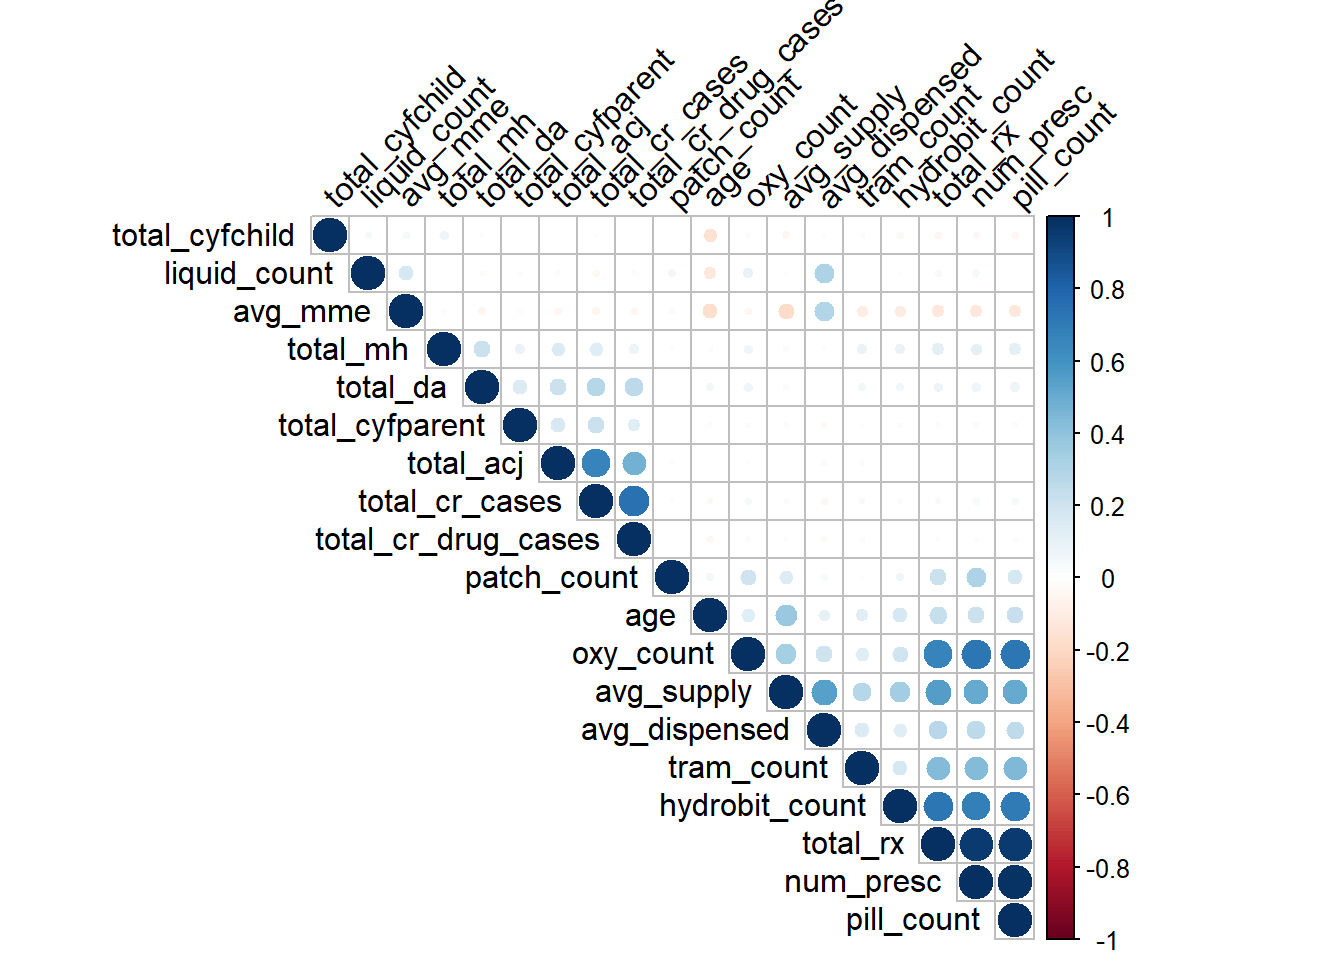
\includegraphics{Total_project_code_files/figure-latex/pressure-1.pdf}

\begin{Shaded}
\begin{Highlighting}[]
\CommentTok{#checking distribution of median_mme, mode_mme, average_mme}

\NormalTok{c1 <-}\StringTok{ }\KeywordTok{ggplot}\NormalTok{(final_data, }\KeywordTok{aes}\NormalTok{(avg_mme)) }\OperatorTok{+}\StringTok{ }\KeywordTok{labs}\NormalTok{(}\DataTypeTok{x=}\StringTok{"Average Morphine Milligram Equivalents (MME)"}\NormalTok{, }\DataTypeTok{y=}\StringTok{"Count"}\NormalTok{) }\OperatorTok{+}\StringTok{ }\KeywordTok{geom_histogram}\NormalTok{(}\DataTypeTok{fill=}\StringTok{"#336B87"}\NormalTok{,}\DataTypeTok{breaks=}\KeywordTok{c}\NormalTok{(}\KeywordTok{seq}\NormalTok{(}\DecValTok{100}\NormalTok{,}\DecValTok{6000}\NormalTok{, }\DataTypeTok{by=}\DecValTok{150}\NormalTok{))) }\OperatorTok{+}\StringTok{ }\KeywordTok{ggtitle}\NormalTok{(}\StringTok{"Average MME Frequency Distribution"}\NormalTok{)}

\NormalTok{c2 <-}\StringTok{ }\KeywordTok{ggplot}\NormalTok{(final_data, }\KeywordTok{aes}\NormalTok{(median_mme)) }\OperatorTok{+}\StringTok{ }\KeywordTok{labs}\NormalTok{(}\DataTypeTok{x=}\StringTok{"Median MME"}\NormalTok{, }\DataTypeTok{y=}\StringTok{"Count"}\NormalTok{) }\OperatorTok{+}\StringTok{ }
\StringTok{  }\KeywordTok{geom_histogram}\NormalTok{(}\DataTypeTok{fill=}\StringTok{"#336B87"}\NormalTok{,}\DataTypeTok{breaks=}\KeywordTok{c}\NormalTok{(}\KeywordTok{seq}\NormalTok{(}\DecValTok{100}\NormalTok{,}\DecValTok{6000}\NormalTok{, }\DataTypeTok{by=}\DecValTok{150}\NormalTok{))) }\OperatorTok{+}\StringTok{ }\KeywordTok{ggtitle}\NormalTok{(}\StringTok{"Median MME Frequency Distribution"}\NormalTok{)}

\NormalTok{c3 <-}\StringTok{ }\KeywordTok{ggplot}\NormalTok{(final_data, }\KeywordTok{aes}\NormalTok{(mode_mme)) }\OperatorTok{+}\StringTok{ }\KeywordTok{labs}\NormalTok{(}\DataTypeTok{x=}\StringTok{"Mode MME"}\NormalTok{, }\DataTypeTok{y=}\StringTok{"Count"}\NormalTok{) }\OperatorTok{+}\StringTok{ }
\StringTok{  }\KeywordTok{geom_histogram}\NormalTok{(}\DataTypeTok{fill=}\StringTok{"#336B87"}\NormalTok{,}\DataTypeTok{breaks=}\KeywordTok{c}\NormalTok{(}\KeywordTok{seq}\NormalTok{(}\DecValTok{100}\NormalTok{,}\DecValTok{6000}\NormalTok{, }\DataTypeTok{by=}\DecValTok{150}\NormalTok{))) }\OperatorTok{+}\StringTok{ }\KeywordTok{ggtitle}\NormalTok{(}\StringTok{"Mode MME Frequency Distribution"}\NormalTok{)}

\KeywordTok{ggarrange}\NormalTok{(c1,c2,c3,}\DataTypeTok{nrow=}\DecValTok{3}\NormalTok{,}\DataTypeTok{ncol=}\DecValTok{1}\NormalTok{)}
\end{Highlighting}
\end{Shaded}

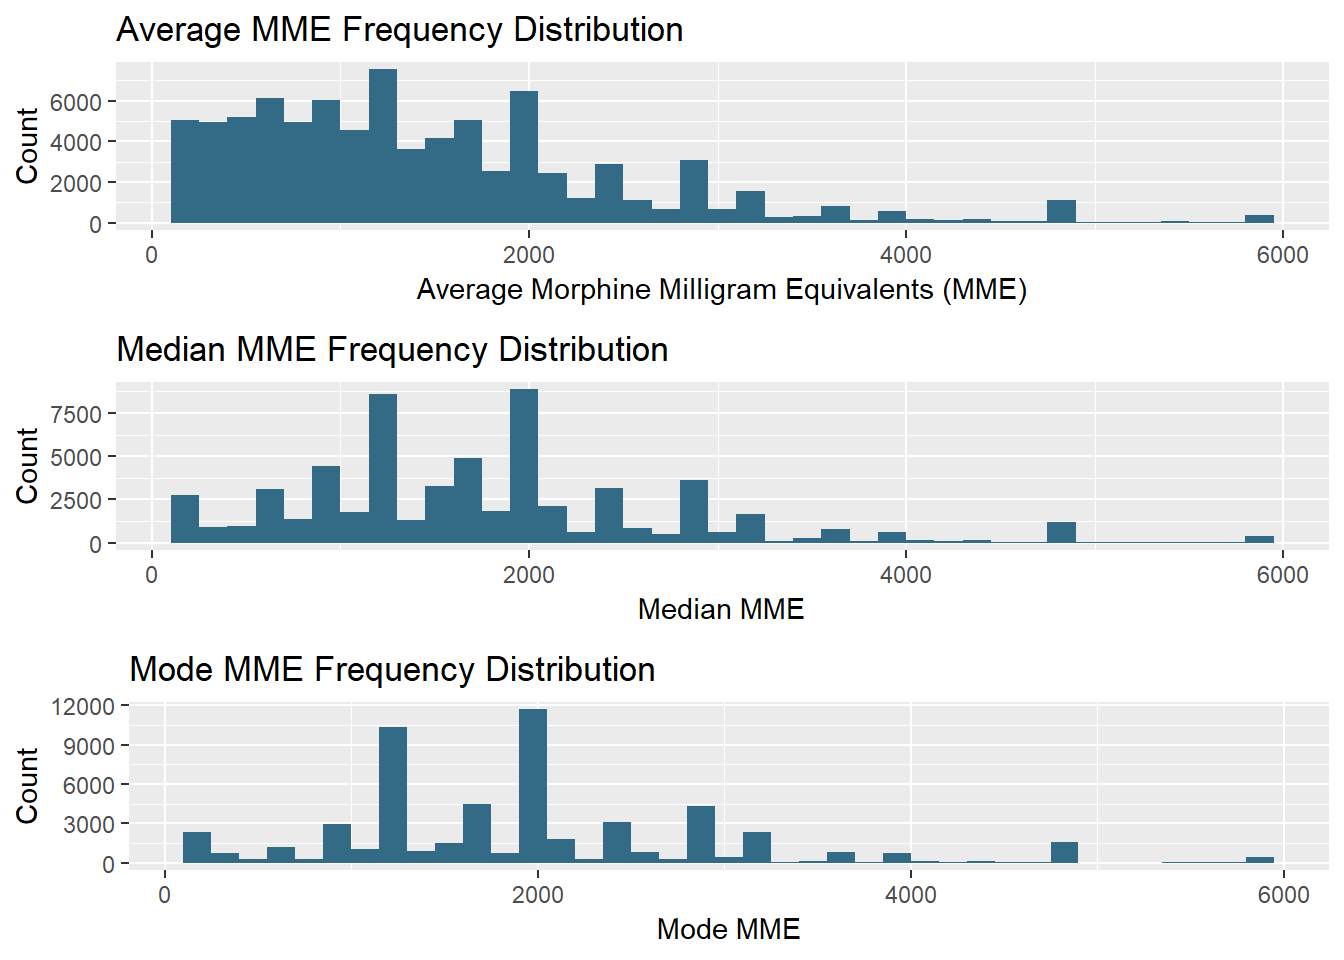
\includegraphics{Total_project_code_files/figure-latex/unnamed-chunk-14-1.pdf}

\begin{Shaded}
\begin{Highlighting}[]
\KeywordTok{rm}\NormalTok{(}\DataTypeTok{list=}\KeywordTok{c}\NormalTok{(}\StringTok{'c1'}\NormalTok{,}\StringTok{'c2'}\NormalTok{,}\StringTok{'c3'}\NormalTok{))}
\end{Highlighting}
\end{Shaded}

median\_mme looks normal and less skewed. We will be using median\_mme
for prediction purpose. Also, we remove columns that are related to
overdose date, for this column is a proxy for the target variable and is
not available in the future dataset.

\begin{Shaded}
\begin{Highlighting}[]
\NormalTok{final_data}\OperatorTok{$}\NormalTok{target <-}\StringTok{ }\OtherTok{NULL}
\NormalTok{final_data}\OperatorTok{$}\NormalTok{target[final_data}\OperatorTok{$}\NormalTok{od_type}\OperatorTok{==}\StringTok{'No Overdose'}\NormalTok{] <-}\StringTok{ }\DecValTok{0}
\NormalTok{final_data}\OperatorTok{$}\NormalTok{target[final_data}\OperatorTok{$}\NormalTok{od_type}\OperatorTok{==}\StringTok{'Non-Opiate Overdose'}\NormalTok{] <-}\StringTok{ }\DecValTok{0}
\NormalTok{final_data}\OperatorTok{$}\NormalTok{target[final_data}\OperatorTok{$}\NormalTok{od_type}\OperatorTok{==}\StringTok{'Opiate Overdose'}\NormalTok{] <-}\StringTok{ }\DecValTok{1}

\CommentTok{#removing columns which are not fit for prediction purpose}
\NormalTok{final_data <-}\StringTok{ }\NormalTok{final_data }\OperatorTok\StringTok{ }\KeywordTok{select}\NormalTok{(}\OperatorTok{-}\KeywordTok{c}\NormalTok{(}\StringTok{'avg_mme'}\NormalTok{,}\StringTok{'mode_mme'}\NormalTok{,}\StringTok{'od_date'}\NormalTok{,}\StringTok{'od_year'}\NormalTok{,}\StringTok{'od_type'}\NormalTok{,}\StringTok{'od_month'}\NormalTok{,}\StringTok{'PERSON_ID'}\NormalTok{))}

\CommentTok{#transforming data using log transformation}
\NormalTok{trans <-}\StringTok{ }\ControlFlowTok{function}\NormalTok{(x)\{}
  \KeywordTok{return}\NormalTok{ (}\KeywordTok{log}\NormalTok{(}\DecValTok{1}\OperatorTok{+}\NormalTok{x))}
\NormalTok{\}}


\CommentTok{#dummifying data to create dummy categorical variables}
\NormalTok{final_df <-}\StringTok{ }\NormalTok{final_data }\OperatorTok\StringTok{ }\KeywordTok{select}\NormalTok{(}\OperatorTok{-}\KeywordTok{c}\NormalTok{(target))}
\NormalTok{final_df <-}\StringTok{ }\KeywordTok{dummify}\NormalTok{(final_df)}
\NormalTok{final_df <-}\StringTok{ }\NormalTok{final_df  }\OperatorTok\StringTok{ }\KeywordTok{mutate_all}\NormalTok{(}\KeywordTok{funs}\NormalTok{(trans))}
\NormalTok{final_df}\OperatorTok{$}\NormalTok{target <-}\StringTok{ }\NormalTok{final_data}\OperatorTok{$}\NormalTok{target}
\end{Highlighting}
\end{Shaded}

\section{Machine Learning Analysis}\label{machine-learning-analysis}

\subsection{Multivariate Logistic
Regression}\label{multivariate-logistic-regression}

\begin{Shaded}
\begin{Highlighting}[]
\CommentTok{#splitting train and testing set (50% ratio)}
\NormalTok{smp_size <-}\StringTok{ }\KeywordTok{floor}\NormalTok{(}\FloatTok{0.5} \OperatorTok{*}\StringTok{ }\KeywordTok{nrow}\NormalTok{(final_df))}
\KeywordTok{set.seed}\NormalTok{(}\DecValTok{1}\NormalTok{)}
\NormalTok{train_indices <-}\StringTok{ }\KeywordTok{sample}\NormalTok{(}\KeywordTok{seq_len}\NormalTok{(}\KeywordTok{nrow}\NormalTok{(final_df)),}\DataTypeTok{size=}\NormalTok{smp_size)}

\NormalTok{xtrain <-}\StringTok{ }\NormalTok{final_df[train_indices,]}
\NormalTok{xtest <-}\StringTok{ }\NormalTok{final_df[}\OperatorTok{-}\NormalTok{train_indices,] }

\NormalTok{xtrain}\OperatorTok{$}\NormalTok{target <-}\StringTok{ }\KeywordTok{factor}\NormalTok{(xtrain}\OperatorTok{$}\NormalTok{target)}
\NormalTok{xtest}\OperatorTok{$}\NormalTok{target <-}\StringTok{ }\KeywordTok{factor}\NormalTok{(xtest}\OperatorTok{$}\NormalTok{target)}

\NormalTok{model_logistic <-}\StringTok{ }\KeywordTok{glm}\NormalTok{ (target}\OperatorTok{~}\NormalTok{., }\DataTypeTok{data=}\NormalTok{xtrain, }\DataTypeTok{family =}\NormalTok{ binomial,}\DataTypeTok{control =} \KeywordTok{list}\NormalTok{(}\DataTypeTok{maxit =} \DecValTok{50}\NormalTok{))}

\NormalTok{## Predict the Values}
\NormalTok{predict_logistic <-}\StringTok{ }\KeywordTok{predict}\NormalTok{(model_logistic, xtest, }\DataTypeTok{type =} \StringTok{'response'}\NormalTok{)}

\NormalTok{## Create Confusion Matrix}
\KeywordTok{table}\NormalTok{(xtest}\OperatorTok{$}\NormalTok{target, predict_logistic }\OperatorTok{>}\StringTok{ }\FloatTok{0.4}\NormalTok{)}
\end{Highlighting}
\end{Shaded}

\begin{verbatim}
##    
##     FALSE
##   0 59787
##   1   538
\end{verbatim}

Due to the fact that we were not able to capture a single opioid
overdose case with logistic regression, we attempt to identify opioid
overdose cases using SMOTE (Synthetic Minority Oversampling Technique).

\subsection{Logistic Regression with
Oversampling}\label{logistic-regression-with-oversampling}

\begin{Shaded}
\begin{Highlighting}[]
\KeywordTok{options}\NormalTok{(}\DataTypeTok{scipen=}\DecValTok{999}\NormalTok{)}

\CommentTok{#performing Oversampling to generate synthetic data}

\KeywordTok{set.seed}\NormalTok{(}\DecValTok{1}\NormalTok{)}
\NormalTok{balanced.data <-}\StringTok{ }\KeywordTok{SMOTE}\NormalTok{(target }\OperatorTok{~}\NormalTok{., xtrain, }\DataTypeTok{perc.over =} \DecValTok{500}\NormalTok{, }\DataTypeTok{k =} \DecValTok{5}\NormalTok{, }\DataTypeTok{perc.under =} \DecValTok{500}\NormalTok{)}
\KeywordTok{as.data.frame}\NormalTok{(}\KeywordTok{table}\NormalTok{(balanced.data}\OperatorTok{$}\NormalTok{target))}
\end{Highlighting}
\end{Shaded}

\begin{verbatim}
##   Var1  Freq
## 1    0 12675
## 2    1  3042
\end{verbatim}

\begin{Shaded}
\begin{Highlighting}[]
\NormalTok{cluster <-}\StringTok{ }\KeywordTok{makeCluster}\NormalTok{(}\KeywordTok{detectCores}\NormalTok{() }\OperatorTok{-}\StringTok{ }\DecValTok{1}\NormalTok{) }\CommentTok{# convention to leave 1 core for OS}
\KeywordTok{registerDoParallel}\NormalTok{(cluster)}


\CommentTok{#instead of training models on all the columns, we are identifying important columns using random forest }
\NormalTok{fitControl <-}\StringTok{ }\KeywordTok{trainControl}\NormalTok{(}\DataTypeTok{method =} \StringTok{"cv"}\NormalTok{, }\DataTypeTok{number =} \DecValTok{5}\NormalTok{, }\DataTypeTok{allowParallel =} \OtherTok{TRUE}\NormalTok{)}

\NormalTok{fit <-}\StringTok{ }\KeywordTok{train}\NormalTok{(target }\OperatorTok{~}\StringTok{ }\NormalTok{., }\DataTypeTok{method=}\StringTok{"rf"}\NormalTok{,}\DataTypeTok{data=}\NormalTok{balanced.data,}\DataTypeTok{trControl =}\NormalTok{ fitControl)}

\NormalTok{var.imp <-}\StringTok{ }\KeywordTok{varImp}\NormalTok{(fit)}
\KeywordTok{plot}\NormalTok{(var.imp,}\DataTypeTok{top=}\DecValTok{15}\NormalTok{)}
\end{Highlighting}
\end{Shaded}

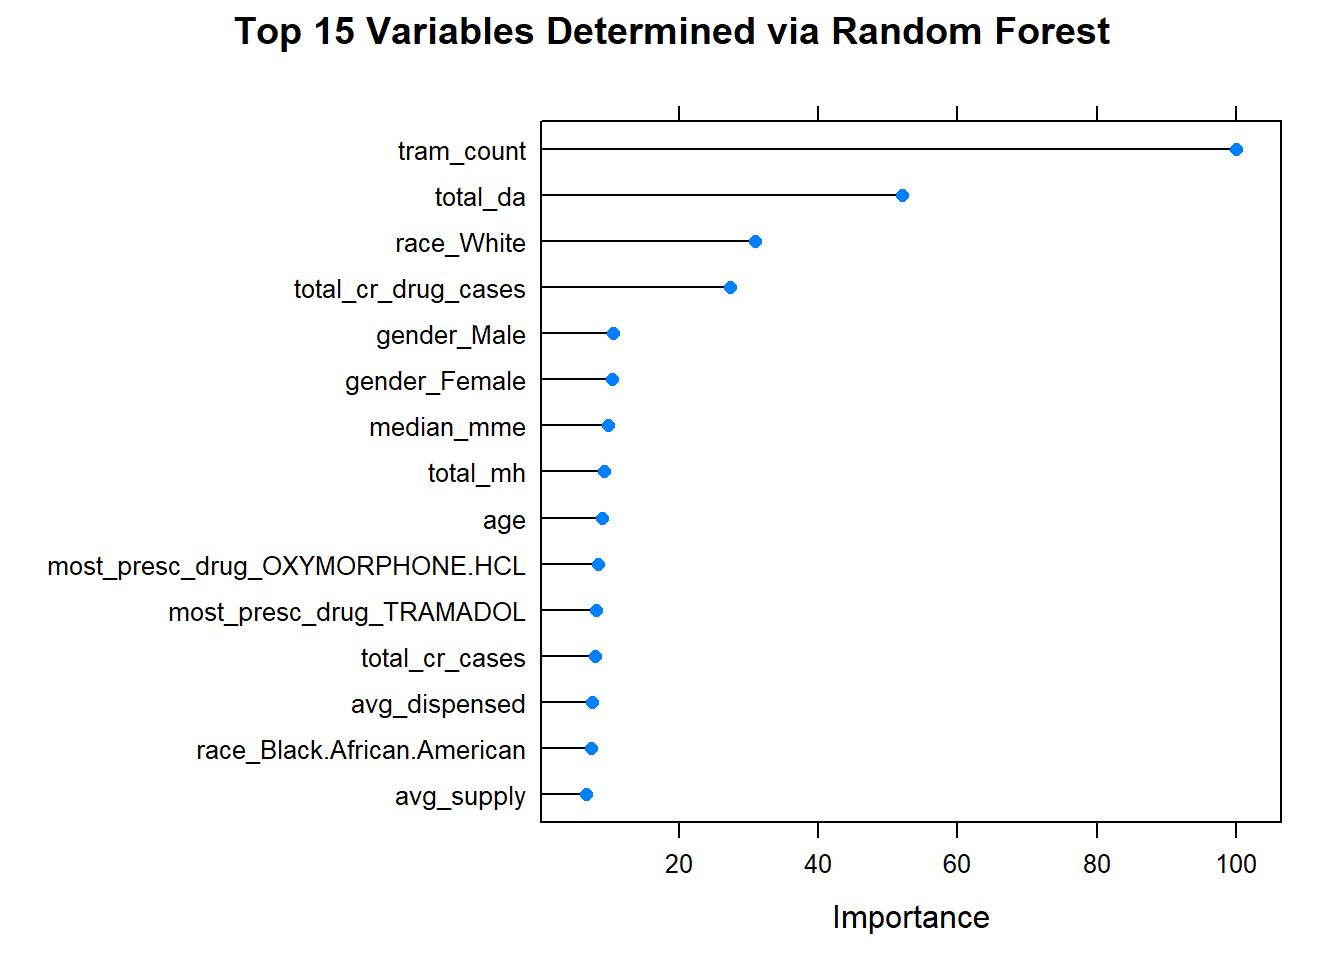
\includegraphics{Total_project_code_files/figure-latex/unnamed-chunk-17-1.pdf}

\subsection{Multivariate Logistic Regression on Selected Features (using
Cross-Validation)}\label{multivariate-logistic-regression-on-selected-features-using-cross-validation}

\begin{Shaded}
\begin{Highlighting}[]
\CommentTok{#selecting columns which turns out to be important in random forest}

\NormalTok{cols_to_select =}\StringTok{ }\KeywordTok{c}\NormalTok{(}\StringTok{"tram_count"}\NormalTok{,}\StringTok{"total_da"}\NormalTok{,}\StringTok{"race_White"}\NormalTok{,}\StringTok{"total_cr_drug_cases"}\NormalTok{,}\StringTok{"median_mme"}\NormalTok{,}\StringTok{"total_cr_cases"}\NormalTok{,}
                   \StringTok{"race_Black.African.American"}\NormalTok{,}\StringTok{"avg_dispensed"}\NormalTok{,}\StringTok{"most_presc_drug_OXYMORPHONE.HCL"}\NormalTok{,}\StringTok{"gender_Male"}\NormalTok{,}\StringTok{"gender_Female"}\NormalTok{,}
                   \StringTok{"avg_supply"}\NormalTok{,}\StringTok{"age"}\NormalTok{,}\StringTok{"total_mh"}\NormalTok{,}\StringTok{"total_acj"}\NormalTok{,}\StringTok{"pill_count"}\NormalTok{,}
                   \StringTok{"num_presc"}\NormalTok{,}\StringTok{"hydrobit_count"}\NormalTok{,}\StringTok{"oxy_count"}\NormalTok{,}\StringTok{"most_presc_drug_HYDROCODONE.BITARTRATE"}\NormalTok{,}\StringTok{"target"}\NormalTok{)}

\NormalTok{xtrain <-}\StringTok{ }\NormalTok{xtrain[,}\KeywordTok{c}\NormalTok{(cols_to_select)]}
\NormalTok{xtest <-}\StringTok{ }\NormalTok{xtest[,}\KeywordTok{c}\NormalTok{(cols_to_select)]}
\NormalTok{balanced.data <-}\StringTok{ }\NormalTok{balanced.data[,}\KeywordTok{c}\NormalTok{(cols_to_select)]}

\CommentTok{#fitting our first model - logistic regression }

\NormalTok{fitControl <-}\StringTok{ }\KeywordTok{trainControl}\NormalTok{(}\DataTypeTok{method =} \StringTok{"repeatedcv"}\NormalTok{,}\DataTypeTok{number =} \DecValTok{5}\NormalTok{,}\DataTypeTok{repeats =} \DecValTok{5}\NormalTok{)}

\NormalTok{model_logistic_cv <-}\StringTok{ }\KeywordTok{train}\NormalTok{(target }\OperatorTok{~}\StringTok{ }\NormalTok{., }\DataTypeTok{data =}\NormalTok{ balanced.data, }\DataTypeTok{method =} \StringTok{"glm"}\NormalTok{,}\DataTypeTok{family =} \KeywordTok{binomial}\NormalTok{(}\DataTypeTok{link =} \StringTok{"logit"}\NormalTok{),}
                          \DataTypeTok{trControl =}\NormalTok{ fitControl)}


\CommentTok{#predicted values for testdata:}
\NormalTok{pred_logistic_cv <-}\StringTok{ }\KeywordTok{predict}\NormalTok{(model_logistic_cv}\OperatorTok{$}\NormalTok{finalModel,xtest,}\DataTypeTok{type =} \StringTok{'response'}\NormalTok{)}

\CommentTok{#test with confusion matrix}
\KeywordTok{table}\NormalTok{(pred_logistic_cv}\OperatorTok{>}\FloatTok{0.4}\NormalTok{,xtest}\OperatorTok{$}\NormalTok{target)}
\end{Highlighting}
\end{Shaded}

\begin{verbatim}
##        
##             0     1
##   FALSE 54759   306
##   TRUE   5028   232
\end{verbatim}

\subsection{Ridge Regression (using
Cross-Validation)}\label{ridge-regression-using-cross-validation}

\begin{Shaded}
\begin{Highlighting}[]
\KeywordTok{set.seed}\NormalTok{(}\DecValTok{123}\NormalTok{) }

\NormalTok{y =}\StringTok{ }\NormalTok{balanced.data}\OperatorTok{$}\NormalTok{target }\OperatorTok\StringTok{ }\KeywordTok{as.matrix}\NormalTok{()}
\NormalTok{x =}\StringTok{ }\NormalTok{balanced.data }\OperatorTok\StringTok{ }\KeywordTok{select}\NormalTok{(}\OperatorTok{-}\KeywordTok{c}\NormalTok{(target))   }\OperatorTok\StringTok{ }\KeywordTok{as.matrix}\NormalTok{()}

\NormalTok{cv.lasso <-}\StringTok{ }\KeywordTok{cv.glmnet}\NormalTok{(x, y, }\DataTypeTok{alpha =} \FloatTok{0.1}\NormalTok{, }\DataTypeTok{family =} \StringTok{"binomial"}\NormalTok{,}\DataTypeTok{nfolds=}\DecValTok{10}\NormalTok{,}\DataTypeTok{type.measure =} \StringTok{"auc"}\NormalTok{)}
\NormalTok{model_ridge <-}\StringTok{ }\KeywordTok{glmnet}\NormalTok{(x, y, }\DataTypeTok{alpha =} \DecValTok{1}\NormalTok{, }\DataTypeTok{family =} \StringTok{"binomial"}\NormalTok{,}\DataTypeTok{lambda =}\NormalTok{ cv.lasso}\OperatorTok{$}\NormalTok{lambda.min)}

\CommentTok{# Make predictions on the test data}
\NormalTok{x.test <-}\StringTok{ }\NormalTok{xtest }\OperatorTok\StringTok{ }\KeywordTok{select}\NormalTok{(}\OperatorTok{-}\KeywordTok{c}\NormalTok{(target)) }\OperatorTok\StringTok{ }\KeywordTok{as.matrix}\NormalTok{()}
\NormalTok{pred_ridge <-}\StringTok{ }\NormalTok{model_ridge }\OperatorTok\StringTok{ }\KeywordTok{predict}\NormalTok{(}\DataTypeTok{newx =}\NormalTok{ x.test)}

\KeywordTok{table}\NormalTok{(pred_ridge}\OperatorTok{>}\FloatTok{0.2}\NormalTok{,xtest}\OperatorTok{$}\NormalTok{target)}
\end{Highlighting}
\end{Shaded}

\begin{verbatim}
##        
##             0     1
##   FALSE 57012   380
##   TRUE   2775   158
\end{verbatim}

\subsection{Random forest (using
Cross-Validation)}\label{random-forest-using-cross-validation}

\begin{Shaded}
\begin{Highlighting}[]
\NormalTok{fitControl <-}\StringTok{ }\KeywordTok{trainControl}\NormalTok{(}\DataTypeTok{method =} \StringTok{"cv"}\NormalTok{, }\DataTypeTok{number =} \DecValTok{10}\NormalTok{, }\DataTypeTok{allowParallel =} \OtherTok{TRUE}\NormalTok{)}

\NormalTok{model_rf <-}\StringTok{ }\KeywordTok{train}\NormalTok{(target }\OperatorTok{~}\StringTok{ }\NormalTok{., }\DataTypeTok{method=}\StringTok{"rf"}\NormalTok{,}\DataTypeTok{data=}\NormalTok{balanced.data,}\DataTypeTok{trControl =}\NormalTok{ fitControl)}

\NormalTok{pred_rf <-}\StringTok{ }\KeywordTok{predict}\NormalTok{(model_logistic_cv}\OperatorTok{$}\NormalTok{finalModel,xtest,}\DataTypeTok{type =} \StringTok{'response'}\NormalTok{)}
\KeywordTok{table}\NormalTok{(pred_rf}\OperatorTok{>}\FloatTok{0.3}\NormalTok{,xtest}\OperatorTok{$}\NormalTok{target)}
\end{Highlighting}
\end{Shaded}

\begin{verbatim}
##        
##             0     1
##   FALSE 52421   235
##   TRUE   7366   303
\end{verbatim}

\subsection{Gradient Boosting Machine (using
Cross-Validation)}\label{gradient-boosting-machine-using-cross-validation}

\begin{Shaded}
\begin{Highlighting}[]
\KeywordTok{set.seed}\NormalTok{(}\DecValTok{123}\NormalTok{)}
\NormalTok{fitControl =}\StringTok{ }\KeywordTok{trainControl}\NormalTok{(}\DataTypeTok{method=}\StringTok{"cv"}\NormalTok{, }\DataTypeTok{number=}\DecValTok{10}\NormalTok{, }\DataTypeTok{returnResamp =} \StringTok{"all"}\NormalTok{,}\DataTypeTok{allowParallel =} \OtherTok{TRUE}\NormalTok{)}

\NormalTok{model_gbm =}\StringTok{ }\KeywordTok{train}\NormalTok{(target}\OperatorTok{~}\NormalTok{., }\DataTypeTok{data=}\NormalTok{balanced.data, }\DataTypeTok{method=}\StringTok{"gbm"}\NormalTok{,}\DataTypeTok{distribution=}\StringTok{"bernoulli"}\NormalTok{, }\DataTypeTok{trControl=}\NormalTok{fitControl, }\DataTypeTok{verbose=}\NormalTok{F, }\DataTypeTok{tuneGrid=}\KeywordTok{data.frame}\NormalTok{(}\DataTypeTok{.n.trees=}\DecValTok{5000}\NormalTok{, }\DataTypeTok{.shrinkage=}\FloatTok{0.1}\NormalTok{, }\DataTypeTok{.interaction.depth=}\DecValTok{1}\NormalTok{, }\DataTypeTok{.n.minobsinnode=}\DecValTok{1}\NormalTok{))}

\NormalTok{pred_gbm <-}\StringTok{ }\KeywordTok{predict}\NormalTok{(model_gbm,xtest,}\DataTypeTok{type =} \StringTok{'prob'}\NormalTok{)}

\KeywordTok{table}\NormalTok{(pred_gbm}\OperatorTok{$}\StringTok{'1'}\OperatorTok{>}\FloatTok{0.2}\NormalTok{,xtest}\OperatorTok{$}\NormalTok{target)}
\end{Highlighting}
\end{Shaded}

\begin{verbatim}
##        
##             0     1
##   FALSE 56983   370
##   TRUE   2804   168
\end{verbatim}

\begin{Shaded}
\begin{Highlighting}[]
\KeywordTok{stopCluster}\NormalTok{(cluster)}
\KeywordTok{registerDoSEQ}\NormalTok{()}
\end{Highlighting}
\end{Shaded}

\subsection{AdaBoost}\label{adaboost}

\begin{Shaded}
\begin{Highlighting}[]
\NormalTok{model_ada =}\StringTok{ }\KeywordTok{ada}\NormalTok{(}\DataTypeTok{formula =}\NormalTok{ target }\OperatorTok{~}\StringTok{ }\NormalTok{.,}\DataTypeTok{data=}\NormalTok{balanced.data ,}\DataTypeTok{iter=}\DecValTok{10}\NormalTok{)}

\NormalTok{pred_ada <-}\StringTok{ }\KeywordTok{predict}\NormalTok{(model_ada,xtest,}\DataTypeTok{type =} \StringTok{'prob'}\NormalTok{)}

\KeywordTok{table}\NormalTok{(pred_ada[,}\DecValTok{2}\NormalTok{]}\OperatorTok{>}\FloatTok{0.2}\NormalTok{,xtest}\OperatorTok{$}\NormalTok{target)}
\end{Highlighting}
\end{Shaded}

\begin{verbatim}
##        
##             0     1
##   FALSE 56033   355
##   TRUE   3754   183
\end{verbatim}

\subsection{Neural Network}\label{neural-network}

\begin{Shaded}
\begin{Highlighting}[]
\CommentTok{# Neural net}

\NormalTok{balanced.data2 <-}\StringTok{ }\KeywordTok{SMOTE}\NormalTok{(target }\OperatorTok{~}\NormalTok{., xtrain, }\DataTypeTok{perc.over =} \DecValTok{4800}\NormalTok{, }\DataTypeTok{k =} \DecValTok{5}\NormalTok{, }\DataTypeTok{perc.under =} \DecValTok{2400}\NormalTok{)}


\NormalTok{y_train <-}\StringTok{ }\KeywordTok{as.numeric}\NormalTok{(balanced.data2}\OperatorTok{$}\NormalTok{target) }\OperatorTok\StringTok{ }\KeywordTok{as.matrix}\NormalTok{()}
\NormalTok{y_test <-}\StringTok{ }\KeywordTok{as.numeric}\NormalTok{(xtest}\OperatorTok{$}\NormalTok{target) }\OperatorTok\StringTok{ }\KeywordTok{as.matrix}\NormalTok{()}

\NormalTok{x_train <-}\StringTok{ }\NormalTok{balanced.data2 }\OperatorTok\StringTok{ }\KeywordTok{select}\NormalTok{(}\OperatorTok{-}\KeywordTok{c}\NormalTok{(target)) }\OperatorTok\StringTok{ }\KeywordTok{as.matrix}\NormalTok{()}
\NormalTok{x_test <-}\StringTok{ }\NormalTok{xtest }\OperatorTok\StringTok{ }\KeywordTok{select}\NormalTok{(}\OperatorTok{-}\KeywordTok{c}\NormalTok{(target)) }\OperatorTok\StringTok{ }\KeywordTok{as.matrix}\NormalTok{()}

\CommentTok{#defining a neural net model}
\NormalTok{model_nn <-}\StringTok{ }\KeywordTok{keras_model_sequential}\NormalTok{() }
\NormalTok{model_nn <-}\StringTok{ }\NormalTok{model_nn }\OperatorTok\StringTok{ }
\StringTok{  }\KeywordTok{layer_dense}\NormalTok{(}\DataTypeTok{units =} \DecValTok{256}\NormalTok{, }\DataTypeTok{activation =} \StringTok{'tanh'}\NormalTok{, }\DataTypeTok{input_shape =} \KeywordTok{c}\NormalTok{(}\DecValTok{20}\NormalTok{)) }\OperatorTok\StringTok{ }
\StringTok{  }\KeywordTok{layer_dropout}\NormalTok{(}\DataTypeTok{rate =} \FloatTok{0.4}\NormalTok{) }\OperatorTok\StringTok{ }
\StringTok{  }\KeywordTok{layer_dense}\NormalTok{( }\DataTypeTok{units=} \DecValTok{256}\NormalTok{, }\DataTypeTok{kernel_initializer =} \StringTok{"uniform"}\NormalTok{, }\DataTypeTok{activation =} \StringTok{"tanh"}\NormalTok{) }\OperatorTok
\StringTok{  }\KeywordTok{layer_dropout}\NormalTok{(}\FloatTok{0.1}\NormalTok{) }\OperatorTok
\StringTok{  }\KeywordTok{layer_dense}\NormalTok{(}\DataTypeTok{units =} \DecValTok{64}\NormalTok{, }\DataTypeTok{activation =} \StringTok{'relu'}\NormalTok{) }\OperatorTok
\StringTok{  }\KeywordTok{layer_dropout}\NormalTok{(}\DataTypeTok{rate =} \FloatTok{0.3}\NormalTok{) }\OperatorTok
\StringTok{  }\KeywordTok{layer_dense}\NormalTok{(}\DataTypeTok{units =} \DecValTok{1}\NormalTok{, }\DataTypeTok{activation =} \StringTok{'softmax'}\NormalTok{)}

\NormalTok{model_nn }\OperatorTok\StringTok{ }\KeywordTok{compile}\NormalTok{(}
  \DataTypeTok{loss =} \StringTok{'binary_crossentropy'}\NormalTok{,}
  \DataTypeTok{optimizer =} \KeywordTok{optimizer_rmsprop}\NormalTok{(),}
  \DataTypeTok{metrics =} \KeywordTok{c}\NormalTok{(}\StringTok{'accuracy'}\NormalTok{)}
\NormalTok{)}

\NormalTok{history <-}\StringTok{ }\NormalTok{model_nn }\OperatorTok\StringTok{ }\KeywordTok{fit}\NormalTok{(}
\NormalTok{  x_train, y_train, }
  \DataTypeTok{epochs =} \DecValTok{30}\NormalTok{, }\DataTypeTok{batch_size =} \DecValTok{128}\NormalTok{, }
  \DataTypeTok{validation_split =} \FloatTok{0.2}
\NormalTok{)}

\NormalTok{pred_model_nn =}\StringTok{ }\NormalTok{model_nn }\OperatorTok\StringTok{ }\KeywordTok{predict}\NormalTok{(x_test)}
\KeywordTok{table}\NormalTok{(pred_model_nn,xtest}\OperatorTok{$}\NormalTok{target)}
\end{Highlighting}
\end{Shaded}

\begin{verbatim}
##              
## pred_model_nn     0     1
##             1 59787   538
\end{verbatim}

\subsection{Evaluation of Machine Learning
Methods}\label{evaluation-of-machine-learning-methods}

\begin{Shaded}
\begin{Highlighting}[]
\CommentTok{#overlapping all the ROC curve}

\KeywordTok{roc}\NormalTok{(xtest}\OperatorTok{$}\NormalTok{target,pred_logistic_cv,}\DataTypeTok{plot=}\OtherTok{TRUE}\NormalTok{,}\DataTypeTok{legacy.axes=}\OtherTok{TRUE}\NormalTok{, }\DataTypeTok{col=}\StringTok{"#377eb8"}\NormalTok{,}
    \DataTypeTok{xlab=}\StringTok{"False Positive Rate"}\NormalTok{,}\DataTypeTok{ylab=}\StringTok{"True Positive Rate"}\NormalTok{)}
\end{Highlighting}
\end{Shaded}

\begin{verbatim}
## 
## Call:
## roc.default(response = xtest$target, predictor = pred_logistic_cv,     plot = TRUE, legacy.axes = TRUE, col = "#377eb8", xlab = "False Positive Rate",     ylab = "True Positive Rate")
## 
## Data: pred_logistic_cv in 59787 controls (xtest$target 0) < 538 cases (xtest$target 1).
## Area under the curve: 0.8468
\end{verbatim}

\begin{Shaded}
\begin{Highlighting}[]
\KeywordTok{plot.roc}\NormalTok{(xtest}\OperatorTok{$}\NormalTok{target,pred_ridge, }\DataTypeTok{col=}\StringTok{"#4daf4a"}\NormalTok{,}\DataTypeTok{add=}\OtherTok{TRUE}\NormalTok{)}
\KeywordTok{plot.roc}\NormalTok{(xtest}\OperatorTok{$}\NormalTok{target,pred_rf, }\DataTypeTok{col=}\StringTok{"#FF420E"}\NormalTok{,}\DataTypeTok{add=}\OtherTok{TRUE}\NormalTok{)}
\KeywordTok{plot.roc}\NormalTok{(xtest}\OperatorTok{$}\NormalTok{target,pred_gbm}\OperatorTok{$}\StringTok{'1'}\NormalTok{, }\DataTypeTok{col=}\StringTok{"#FFBB00"}\NormalTok{,}\DataTypeTok{add=}\OtherTok{TRUE}\NormalTok{)}
\KeywordTok{plot.roc}\NormalTok{(xtest}\OperatorTok{$}\NormalTok{target,pred_ada[,}\DecValTok{2}\NormalTok{], }\DataTypeTok{col=}\StringTok{"#763626"}\NormalTok{,}\DataTypeTok{add=}\OtherTok{TRUE}\NormalTok{)}
\KeywordTok{plot.roc}\NormalTok{(xtest}\OperatorTok{$}\NormalTok{target,pred_model_nn, }\DataTypeTok{col=}\StringTok{"#375E97"}\NormalTok{,}\DataTypeTok{add=}\OtherTok{TRUE}\NormalTok{)}

\KeywordTok{legend}\NormalTok{(}\StringTok{"bottomright"}\NormalTok{,}\DataTypeTok{legend=}\KeywordTok{c}\NormalTok{(}
  \KeywordTok{paste}\NormalTok{(}\StringTok{"Logistic regression (LR), AUC = "}\NormalTok{, }\KeywordTok{format}\NormalTok{(}\KeywordTok{roc}\NormalTok{(xtest}\OperatorTok{$}\NormalTok{target,pred_logistic_cv)}\OperatorTok{$}\NormalTok{auc,}\DataTypeTok{digits=}\DecValTok{2}\NormalTok{)), }
  \KeywordTok{paste}\NormalTok{(}\StringTok{"Ridge LR, AUC = "}\NormalTok{, }\KeywordTok{format}\NormalTok{(}\KeywordTok{roc}\NormalTok{(xtest}\OperatorTok{$}\NormalTok{target,pred_ridge)}\OperatorTok{$}\NormalTok{auc, }\DataTypeTok{digits=}\DecValTok{2}\NormalTok{)),}
  \KeywordTok{paste}\NormalTok{(}\StringTok{"Random Forest, AUC = "}\NormalTok{, }\KeywordTok{format}\NormalTok{(}\KeywordTok{roc}\NormalTok{(xtest}\OperatorTok{$}\NormalTok{target,pred_rf)}\OperatorTok{$}\NormalTok{auc, }\DataTypeTok{digits=}\DecValTok{2}\NormalTok{)),}
  \KeywordTok{paste}\NormalTok{(}\StringTok{"Gradient Boosting, AUC = "}\NormalTok{, }\KeywordTok{format}\NormalTok{(}\KeywordTok{roc}\NormalTok{(xtest}\OperatorTok{$}\NormalTok{target,pred_gbm}\OperatorTok{$}\StringTok{'1'}\NormalTok{)}\OperatorTok{$}\NormalTok{auc, }\DataTypeTok{digits=}\DecValTok{2}\NormalTok{)),}
  \KeywordTok{paste}\NormalTok{(}\StringTok{"AdaBoost, AUC = "}\NormalTok{, }\KeywordTok{format}\NormalTok{(}\KeywordTok{roc}\NormalTok{(xtest}\OperatorTok{$}\NormalTok{target,pred_ada[,}\DecValTok{2}\NormalTok{])}\OperatorTok{$}\NormalTok{auc, }\DataTypeTok{digits=}\DecValTok{2}\NormalTok{)),}
  \KeywordTok{paste}\NormalTok{(}\StringTok{"Neural Network, AUC = "}\NormalTok{, }\KeywordTok{format}\NormalTok{(}\KeywordTok{roc}\NormalTok{(xtest}\OperatorTok{$}\NormalTok{target,pred_model_nn)}\OperatorTok{$}\NormalTok{auc, }\DataTypeTok{digits=}\DecValTok{2}\NormalTok{ ))),}
            \DataTypeTok{col=}\KeywordTok{c}\NormalTok{(}\StringTok{"#377eb8"}\NormalTok{,}\StringTok{"#4daf4a"}\NormalTok{,}\StringTok{"#FF420E"}\NormalTok{,}\StringTok{"#FFBB00"}\NormalTok{,}\StringTok{"#763626"}\NormalTok{,}\StringTok{"#375E97"}\NormalTok{),}\DataTypeTok{lwd=}\DecValTok{4}\NormalTok{, }\DataTypeTok{bg=}\NormalTok{F, }\DataTypeTok{cex=}\FloatTok{0.75}\NormalTok{, }\DataTypeTok{bty=}\StringTok{"n"}\NormalTok{)}
\end{Highlighting}
\end{Shaded}

\includegraphics{Total_project_code_files/figure-latex/unnamed-chunk-24-1.pdf}

\section{Survival Analysis}\label{survival-analysis}

\subsection{Survival Analysis: Kaplan Meier (All
Individuals)}\label{survival-analysis-kaplan-meier-all-individuals}

\begin{Shaded}
\begin{Highlighting}[]
\CommentTok{# first step in creating the "time" variable }
\CommentTok{# this will be the sequence of months since joining the dataset for each individual}
\NormalTok{prog =}\StringTok{ }\NormalTok{prog }\OperatorTok\StringTok{ }\KeywordTok{group_by}\NormalTok{(PERSON_ID) }\OperatorTok\StringTok{ }\KeywordTok{mutate}\NormalTok{(}\DataTypeTok{start_year=}\KeywordTok{min}\NormalTok{(YEAR))}
\NormalTok{prog =}\StringTok{ }\NormalTok{prog }\OperatorTok\StringTok{ }\KeywordTok{mutate}\NormalTok{(}\DataTypeTok{months =}\NormalTok{ (YEAR}\OperatorTok\NormalTok{start_year}\OperatorTok{*}\DecValTok{12}\NormalTok{) }\OperatorTok{+}\StringTok{ }\NormalTok{MONTH)}
\NormalTok{prog =}\StringTok{ }\NormalTok{prog }\OperatorTok\StringTok{ }\KeywordTok{group_by}\NormalTok{(PERSON_ID) }\OperatorTok\StringTok{ }\KeywordTok{mutate}\NormalTok{(}\DataTypeTok{min_month_year =} \KeywordTok{min}\NormalTok{(months))}
\NormalTok{prog =}\StringTok{ }\NormalTok{prog }\OperatorTok\StringTok{ }\KeywordTok{mutate}\NormalTok{(}\DataTypeTok{month_seq =}\NormalTok{ months }\OperatorTok{-}\StringTok{ }\NormalTok{min_month_year }\OperatorTok{+}\StringTok{ }\DecValTok{1}\NormalTok{)}

\CommentTok{# first step in creating the "status" variable}
\CommentTok{# this will be the month (in the sequence) when the individual overdosed}
\CommentTok{# it will be NA if the person did not overdose}
\NormalTok{prog}\OperatorTok{$}\NormalTok{od_year_month =}\StringTok{ }\NormalTok{(}\KeywordTok{as.integer}\NormalTok{(prog}\OperatorTok{$}\NormalTok{OVERDOSE_YEAR)}\OperatorTok\NormalTok{prog}\OperatorTok{$}\NormalTok{start_year)}\OperatorTok{*}\DecValTok{12}\OperatorTok{+}\KeywordTok{as.integer}\NormalTok{(prog}\OperatorTok{$}\NormalTok{OVERDOSE_MONTH)}
\NormalTok{prog}\OperatorTok{$}\NormalTok{od_seq =}\StringTok{ }\NormalTok{prog}\OperatorTok{$}\NormalTok{od_year_month }\OperatorTok{-}\StringTok{ }\NormalTok{prog}\OperatorTok{$}\NormalTok{min_month_year }\OperatorTok{+}\StringTok{ }\DecValTok{1}

\CommentTok{# creating the data for survival analysis}
\CommentTok{# one row per individual}
\CommentTok{# time is the last month (in sequence) in which the individual is seen in the dataset }
\CommentTok{# status is whether or not the event (overdose) occurred}
\NormalTok{survival_data =}\StringTok{ }\NormalTok{prog }\OperatorTok\StringTok{ }\KeywordTok{group_by}\NormalTok{(PERSON_ID) }\OperatorTok\StringTok{ }\KeywordTok{summarise}\NormalTok{(}\DataTypeTok{time_yearmonth =} \KeywordTok{max}\NormalTok{(month_seq), }\DataTypeTok{od_time =} \KeywordTok{max}\NormalTok{(od_seq))}
\NormalTok{survival_data =}\StringTok{ }\NormalTok{survival_data }\OperatorTok\StringTok{ }\KeywordTok{mutate}\NormalTok{(}\DataTypeTok{status =} \KeywordTok{if_else}\NormalTok{(}\KeywordTok{is.na}\NormalTok{(od_time), }\DecValTok{0}\NormalTok{, }\DecValTok{1}\NormalTok{))}
\NormalTok{survival_data =}\StringTok{ }\NormalTok{survival_data }\OperatorTok\StringTok{ }\KeywordTok{mutate}\NormalTok{(}\DataTypeTok{time =} \KeywordTok{if_else}\NormalTok{(}\KeywordTok{is.na}\NormalTok{(od_time), time_yearmonth, od_time))}
\NormalTok{survival_data =}\StringTok{ }\NormalTok{survival_data }\OperatorTok\StringTok{ }\KeywordTok{select}\NormalTok{(PERSON_ID, status, time)}
\NormalTok{survival_data =}\StringTok{ }\KeywordTok{merge}\NormalTok{(survival_data, dem, }\DataTypeTok{key=}\StringTok{"PERSON_ID"}\NormalTok{)}
\NormalTok{survival_data =}\StringTok{ }\KeywordTok{merge}\NormalTok{(survival_data, age_df }\OperatorTok\StringTok{ }\KeywordTok{select}\NormalTok{(PERSON_ID, age), }\DataTypeTok{key=}\StringTok{"PERSON_ID"}\NormalTok{)}

\CommentTok{#plot 1 (overall kaplan meier curve)}
\NormalTok{km =}\StringTok{ }\KeywordTok{Surv}\NormalTok{(survival_data}\OperatorTok{$}\NormalTok{time, survival_data}\OperatorTok{$}\NormalTok{status) }\OperatorTok
\StringTok{  }\NormalTok{(}\ControlFlowTok{function}\NormalTok{(x) }\KeywordTok{survfit}\NormalTok{(x }\OperatorTok{~}\StringTok{ }\DecValTok{1}\NormalTok{, }\DataTypeTok{data=}\NormalTok{survival_data))(.)}
\CommentTok{# Kaplan-Meier curve}
\KeywordTok{plot}\NormalTok{(km, }\DataTypeTok{xlab=} \StringTok{"Months In System"}\NormalTok{,}\DataTypeTok{ylab=}\StringTok{"P(survive)"}\NormalTok{, }\DataTypeTok{mark.time=}\NormalTok{T)}
\end{Highlighting}
\end{Shaded}

\includegraphics{Total_project_code_files/figure-latex/unnamed-chunk-25-1.pdf}

\begin{Shaded}
\begin{Highlighting}[]
\NormalTok{km}
\end{Highlighting}
\end{Shaded}

\begin{verbatim}
## Call: survfit(formula = x ~ 1, data = survival_data)
## 
##       n  events  median 0.95LCL 0.95UCL 
##  120650    1222     110      NA      NA
\end{verbatim}

\begin{Shaded}
\begin{Highlighting}[]
\CommentTok{#plot 2 (by gender)}
\NormalTok{km_gender =}\StringTok{ }\KeywordTok{survfit}\NormalTok{(}\KeywordTok{Surv}\NormalTok{(survival_data}\OperatorTok{$}\NormalTok{time, survival_data}\OperatorTok{$}\NormalTok{status) }\OperatorTok{~}\StringTok{ }\NormalTok{gender, }\DataTypeTok{data=}\NormalTok{survival_data)}
\KeywordTok{plot}\NormalTok{(km_gender,}
     \DataTypeTok{col=}\KeywordTok{c}\NormalTok{(}\DecValTok{1}\OperatorTok{:}\DecValTok{3}\NormalTok{), }\DataTypeTok{mark.time =}\NormalTok{ T); }\KeywordTok{legend}\NormalTok{(}\StringTok{"bottomleft"}\NormalTok{, }\KeywordTok{c}\NormalTok{(}\StringTok{"Female"}\NormalTok{,}\StringTok{"Male"}\NormalTok{, }\StringTok{"No Data & Other"}\NormalTok{), }\DataTypeTok{col=}\DecValTok{1}\OperatorTok{:}\DecValTok{3}\NormalTok{, }\DataTypeTok{lty=}\KeywordTok{c}\NormalTok{(}\DecValTok{1}\NormalTok{,}\DecValTok{1}\NormalTok{))}
\end{Highlighting}
\end{Shaded}

\includegraphics{Total_project_code_files/figure-latex/unnamed-chunk-25-2.pdf}

\begin{Shaded}
\begin{Highlighting}[]
\NormalTok{km_gender}
\end{Highlighting}
\end{Shaded}

\begin{verbatim}
## Call: survfit(formula = Surv(survival_data$time, survival_data$status) ~ 
##     gender, data = survival_data)
## 
##                              n events median 0.95LCL 0.95UCL
## gender=Female            73582    515    110      NA      NA
## gender=Male              46857    705     NA      NA      NA
## gender=No Data and Other   211      2     NA     105      NA
\end{verbatim}

\begin{Shaded}
\begin{Highlighting}[]
\CommentTok{#plot 3 (by race but only subsetting to white and black/african-american)}
\NormalTok{survival_data_subset =}\StringTok{ }\NormalTok{survival_data }\OperatorTok\StringTok{ }\KeywordTok{filter}\NormalTok{(race}\OperatorTok{==}\KeywordTok{c}\NormalTok{(}\StringTok{"White"}\NormalTok{, }\StringTok{"Black/African-American"}\NormalTok{))}
\NormalTok{km_race =}\StringTok{ }\KeywordTok{survfit}\NormalTok{(}\KeywordTok{Surv}\NormalTok{(survival_data_subset}\OperatorTok{$}\NormalTok{time, survival_data_subset}\OperatorTok{$}\NormalTok{status) }\OperatorTok{~}\StringTok{ }\NormalTok{race, }\DataTypeTok{data=}\NormalTok{survival_data_subset)}
\KeywordTok{plot}\NormalTok{(km_race,}
     \DataTypeTok{col=}\KeywordTok{c}\NormalTok{(}\DecValTok{1}\OperatorTok{:}\DecValTok{2}\NormalTok{), }\DataTypeTok{mark.time =}\NormalTok{ T); }\KeywordTok{legend}\NormalTok{(}\StringTok{"bottomleft"}\NormalTok{, }\KeywordTok{c}\NormalTok{(}\StringTok{"Black/African-American"}\NormalTok{,}\StringTok{"White"}\NormalTok{), }\DataTypeTok{col=}\DecValTok{1}\OperatorTok{:}\DecValTok{2}\NormalTok{, }\DataTypeTok{lty=}\KeywordTok{c}\NormalTok{(}\DecValTok{1}\NormalTok{,}\DecValTok{1}\NormalTok{))}
\end{Highlighting}
\end{Shaded}

\includegraphics{Total_project_code_files/figure-latex/unnamed-chunk-25-3.pdf}

\begin{Shaded}
\begin{Highlighting}[]
\NormalTok{km_race}
\end{Highlighting}
\end{Shaded}

\begin{verbatim}
## Call: survfit(formula = Surv(survival_data_subset$time, survival_data_subset$status) ~ 
##     race, data = survival_data_subset)
## 
##                                 n events median 0.95LCL 0.95UCL
## race=Black/African-American 20362    100     NA      NA      NA
## race=White                  28574    485    110      NA      NA
\end{verbatim}

\subsection{Survival Analysis: Cox Proportional Hazards Model (All
Individuals)}\label{survival-analysis-cox-proportional-hazards-model-all-individuals}

\begin{Shaded}
\begin{Highlighting}[]
\CommentTok{# Cox model}
\NormalTok{cm =}\StringTok{ }\KeywordTok{Surv}\NormalTok{(survival_data}\OperatorTok{$}\NormalTok{time, survival_data}\OperatorTok{$}\NormalTok{status) }\OperatorTok
\StringTok{  }\NormalTok{(}\ControlFlowTok{function}\NormalTok{(x) }\KeywordTok{coxph}\NormalTok{(x }\OperatorTok{~}\StringTok{ }\NormalTok{age }\OperatorTok{+}\StringTok{ }\NormalTok{gender, }\DataTypeTok{data=}\NormalTok{survival_data))(.)}
\NormalTok{cm}
\end{Highlighting}
\end{Shaded}

\begin{verbatim}
## Call:
## coxph(formula = x ~ age + gender, data = survival_data)
## 
##                            coef exp(coef) se(coef)    z
## age                     0.02728   1.02765  0.00205 13.3
## genderMale              0.63275   1.88279  0.05821 10.9
## genderNo Data and Other 1.49074   4.44038  0.70862  2.1
##                                           p
## age                     <0.0000000000000002
## genderMale              <0.0000000000000002
## genderNo Data and Other               0.035
## 
## Likelihood ratio test=321.4  on 3 df, p=<0.0000000000000002
## n= 120650, number of events= 1222
\end{verbatim}

\begin{Shaded}
\begin{Highlighting}[]
\CommentTok{# Regularized Cox model}
\NormalTok{cox_data =}\StringTok{ }\NormalTok{survival_data }\OperatorTok\StringTok{ }\KeywordTok{select}\NormalTok{(}\OperatorTok{-}\NormalTok{time, }\OperatorTok{-}\NormalTok{status, }\OperatorTok{-}\NormalTok{PERSON_ID) }\OperatorTok\StringTok{ }\KeywordTok{as.data.frame}\NormalTok{() }\OperatorTok\StringTok{ }\KeywordTok{as.matrix}\NormalTok{()}
\NormalTok{cox_data =}\StringTok{ }\NormalTok{cox_data }\OperatorTok\StringTok{ }\KeywordTok{dummy_cols}\NormalTok{(}\KeywordTok{c}\NormalTok{(}\StringTok{"gender"}\NormalTok{, }\StringTok{"race"}\NormalTok{))}
\NormalTok{cox_data =}\StringTok{ }\NormalTok{cox_data }\OperatorTok\StringTok{ }\KeywordTok{select}\NormalTok{(}\OperatorTok{-}\NormalTok{gender, }\OperatorTok{-}\NormalTok{race) }\OperatorTok\StringTok{ }\KeywordTok{as.data.frame}\NormalTok{() }\OperatorTok\StringTok{ }\KeywordTok{as.matrix}\NormalTok{()}
\NormalTok{lm =}\StringTok{ }\KeywordTok{glmnet}\NormalTok{(cox_data, }\KeywordTok{Surv}\NormalTok{(survival_data}\OperatorTok{$}\NormalTok{time, survival_data}\OperatorTok{$}\NormalTok{status), }\DataTypeTok{family=}\StringTok{"cox"}\NormalTok{)}
\KeywordTok{plot}\NormalTok{(lm)}
\end{Highlighting}
\end{Shaded}

\includegraphics{Total_project_code_files/figure-latex/unnamed-chunk-26-1.pdf}

\begin{Shaded}
\begin{Highlighting}[]
\CommentTok{# Choosing s using cross validation}
\NormalTok{cvlm =}\StringTok{ }\KeywordTok{cv.glmnet}\NormalTok{(cox_data, }\KeywordTok{Surv}\NormalTok{(survival_data}\OperatorTok{$}\NormalTok{time, survival_data}\OperatorTok{$}\NormalTok{status), }\DataTypeTok{family=}\StringTok{"cox"}\NormalTok{)}
\KeywordTok{plot}\NormalTok{(cvlm)}
\end{Highlighting}
\end{Shaded}

\includegraphics{Total_project_code_files/figure-latex/unnamed-chunk-26-2.pdf}

\begin{Shaded}
\begin{Highlighting}[]
\CommentTok{# showing coefficients of model with minimum lambda}
\KeywordTok{coef}\NormalTok{(lm, }\DataTypeTok{s=}\NormalTok{cvlm}\OperatorTok{$}\NormalTok{lambda.min)}
\end{Highlighting}
\end{Shaded}

\begin{verbatim}
## 10 x 1 sparse Matrix of class "dgCMatrix"
##                                               1
## age                                  0.02688772
## gender_Female                       -0.61583464
## gender_Male                          .         
## gender_No Data and Other             1.26944943
## race_White                           1.15013650
## race_Black/African-American         -0.11610053
## race_Biracial/Multiracial            0.53617128
## race_No Data and Other               .         
## race_Asian                          -0.42251671
## race_American Indian/Alaskan Native -1.01009300
\end{verbatim}

\begin{Shaded}
\begin{Highlighting}[]
\CommentTok{# showing coefficients of model with lambda within 1se}
\KeywordTok{coef}\NormalTok{(lm, }\DataTypeTok{s=}\NormalTok{cvlm}\OperatorTok{$}\NormalTok{lambda.1se)}
\end{Highlighting}
\end{Shaded}

\begin{verbatim}
## 10 x 1 sparse Matrix of class "dgCMatrix"
##                                              1
## age                                  0.0160821
## gender_Female                       -0.3608499
## gender_Male                          .        
## gender_No Data and Other             .        
## race_White                           0.8427408
## race_Black/African-American          .        
## race_Biracial/Multiracial            .        
## race_No Data and Other               .        
## race_Asian                           .        
## race_American Indian/Alaskan Native  .
\end{verbatim}

Need to see if/how this changes if everyone has the same starting point.
So, decided to do the survival analysis for a specific cohort i.e.~same
starting point. We chose cohort==2009 because it has the most amount of
data available longitudinally.


\end{document}
